\documentclass[UTF8,a4paper]{article}
\usepackage{array}
\usepackage{amsmath}
\usepackage{listings}
\usepackage{graphicx}
\usepackage{subcaption}
\usepackage{color} %red, green, blue, yellow, cyan, magenta, black, white
\definecolor{mygreen}{RGB}{28,172,0} % color values Red, Green, Blue
\definecolor{mylilas}{RGB}{170,55,241}
\usepackage{geometry}
\geometry{left=2.0cm,right=2.0cm,top=2.0cm,bottom=2.0cm}

\renewcommand{\theequation}{\arabic{section}.\arabic{equation}}
\renewcommand{\thefigure}{\arabic{section}.\arabic{figure}}
\renewcommand{\thetable}{\arabic{section}.\arabic{table}}
\makeatletter
\@addtoreset{equation}{section}
\@addtoreset{figure}{section}
\@addtoreset{table}{section}
\makeatother

\title{Digital Image Processing 2017fall \\ Project Report }
\author{Name: Wang Yiqing \\ Student Number: 515 030 910 456 \\ Email: WangYiqing\_2015@sjtu.edu.cn}
\date{2017-12-10}

\begin{document}
\maketitle

\clearpage
\tableofcontents
\clearpage


\lstset{language=Matlab,%
    %basicstyle=\color{red},
    frame=single, %设置边框格式
    breaklines=true,%
    morekeywords={matlab2tikz},
    keywordstyle=\color{blue},%
    morekeywords=[2]{1}, keywordstyle=[2]{\color{black}},
    identifierstyle=\color{black},%
    stringstyle=\color{mylilas},
    commentstyle=\color{mygreen},%
    showstringspaces=false,%without this there will be a symbol in the places where there is a space
    numbers=left,%
    numberstyle={\tiny \color{black}},% size of the numbers
    numbersep=9pt, % this defines how far the numbers are from the text
    emph=[1]{for,end,break},emphstyle=[1]\color{blue}, %some words to emphasise
    %emph=[2]{word1,word2}, emphstyle=[2]{style},    
}

\section{Project 1 - Histogram Equalization}

\subsection{Project Proposal}
In this project we implement histogram equalization. First, plot the histogram of an image, then implement histogram equalization and display the equalized image and histogram. Test images are \emph{Fig1.jpg, Fig2.jpg}.

\subsection{Preliminaries}
Let $r$ denote the intensity of a pixel in the original image and $r \in [0,L-1]$. We consider a transformation \begin{equation}s=T(r) ~~~~ 0 \leq r \leq L-1 \end{equation} that produce an output intensity level $s$ for every pixel in the input image having intensity $r$. We assume that:
\\ \textbf{(a)} $T(r)$ is a monotonically increasing function in the interval $0 \leq r \leq L-1$; and \\
\textbf{(b)} $0 \leq T(r) \leq L-1$ for $r \in [0, L-1]$. \\
Condition \textbf{(a)} and \textbf{(b)} guarantee the existing of inverse function $r=T^{-1}(s)$ which is monotonically increasing. 
The central idea is that \emph{intensity levels of an image can be viewed as random variables in the interval $[0, L-1]$ and can be described by probability density function (PDF).} Let $p_r(r)$ and $p_s(s)$ to be the PDF of $r$ and $s$ respectively. Thus we can apply the basic result of probability theory that \emph{if $T(r)$ is differentiable over the range of interest, we have this below relationship between $p_r(r)$ and $p_s(s)$: }
\begin{equation} p_s(s)=p_r(r) \left| \frac{dr}{ds} \right| \label{equ:basicprob} \end{equation}
Then consider the cumulative distribution function(CDF) which is exactly used here as the transformation function $T(r)$ \begin{equation} s=T(r)=(L-1) \int_0^r p_r(w)dw  \label{equ:histEquTrans} \end{equation}
Now we are ready to prove the transformation really does the histogram equalization. Firstly, compute the derivatives. The last $=$ is from the assumption \textbf{(a)} stating the monotonically increasing.
\begin{equation} \frac{ds}{dr}=\frac{dT(r)}{dr}=(L-1)p_r(r) = \left| \frac{ds}{dr} \right| \end{equation}
Thus, substituting the result for Eq.\ref{equ:basicprob}, we get the desired result
\begin{equation} p_s(s) = p_r(r) \frac{1}{(L-1)p_r(r)} = \frac{1}{L-1} \end{equation}
which show $p_s(s)$ follows uniform distribution.

\subsection{Histogram equalization}
Histogram equalization on an image of size $M\times N$ is like a discrete version of the process in the preliminaries section. \begin{equation} p_r(r_k)=\frac{n_k}{MN} ~~~~~~ k=0,1,2,...,L-1  \end{equation} where $n_k$ is the number of pixels that have intensity $r_k$. The discrete form of Eq.\ref{equ:histEquTrans} is \begin{equation} s_k=T(r_k)=(L-1)\sum_{j=0}^k p_r(r_j)=\frac{L-1}{MN} \sum_{j=0}^k n_k ~~~~~~ k=0,1,2,...,L-1 \end{equation}
Based on these discrete form equation, I implement the matlab function and test them on \emph{Fig1.jpg, Fig2.jpg} and get the results listed in \ref{fig:result1} and \ref{fig:result2} respectively.
\begin{figure}[h!]
	\centering
	\begin{subfigure}[b]{0.45\linewidth}
		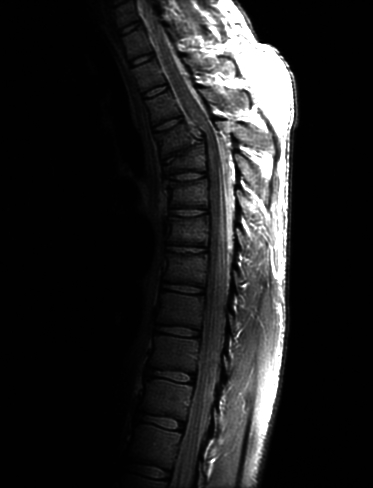
\includegraphics[width=\linewidth]{myfigure/p1/Fig1.jpg}
		\caption{}
		\label{fig:Fig1}
	\end{subfigure}
  	\begin{subfigure}[b]{0.45\linewidth}
		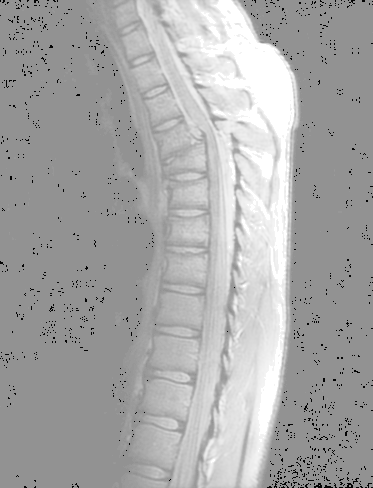
\includegraphics[width=\linewidth]{myfigure/p1/g1.png}
		\caption{}
		\label{fig:g1}
	\end{subfigure}
	\begin{subfigure}[b]{0.45\linewidth}
    	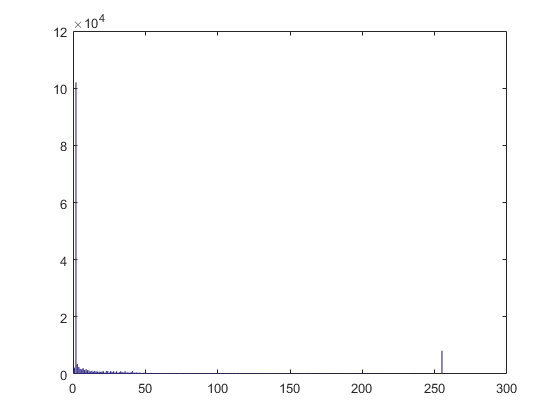
\includegraphics[width=\linewidth]{myfigure/p1/fbar1.png}
    	\caption{}
    	\label{fig:fbar1}
  	\end{subfigure}
	\begin{subfigure}[b]{0.45\linewidth}
    	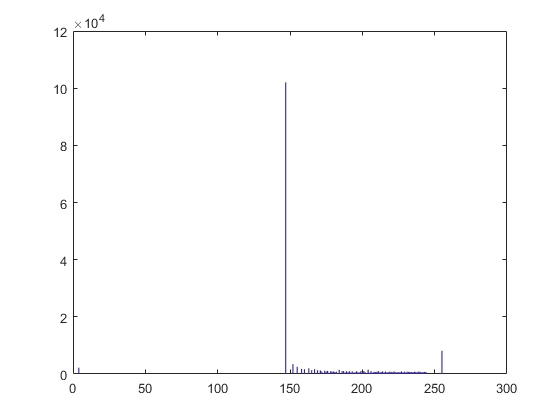
\includegraphics[width=\linewidth]{myfigure/p1/gbar1.png}
    	\caption{}
    	\label{fig:gbar1}
  	\end{subfigure}
  	\caption{Results of Fig1.jpg. (a)Original image. (b)Processed image after applying histogram equalization. (c)Histogram of original image. (d)Histogram of processed image.}
  	\label{fig:result1}
\end{figure}

\begin{figure}[h!]
	\centering
	\begin{subfigure}[b]{0.45\linewidth}
		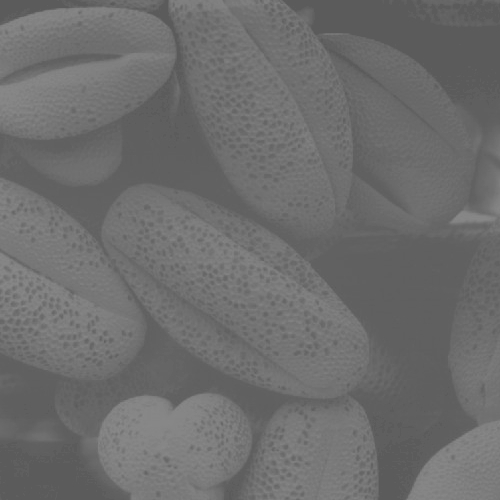
\includegraphics[width=\linewidth]{myfigure/p1/Fig2.jpg}
		\caption{}
		\label{fig:Fig2}
	\end{subfigure}
	\begin{subfigure}[b]{0.45\linewidth}
		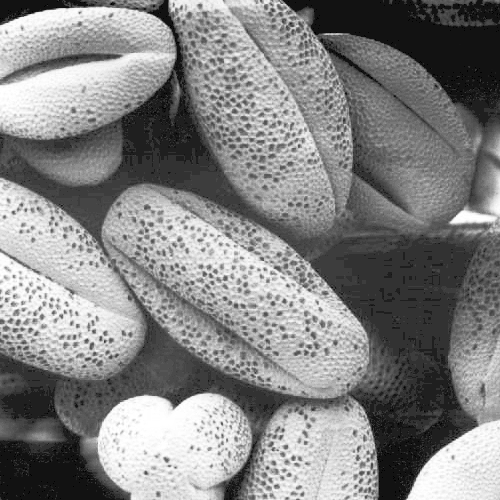
\includegraphics[width=\linewidth]{myfigure/p1/g2.png}
		\caption{}
		\label{fig:g2}
	\end{subfigure}
	\begin{subfigure}[b]{0.45\linewidth}
    	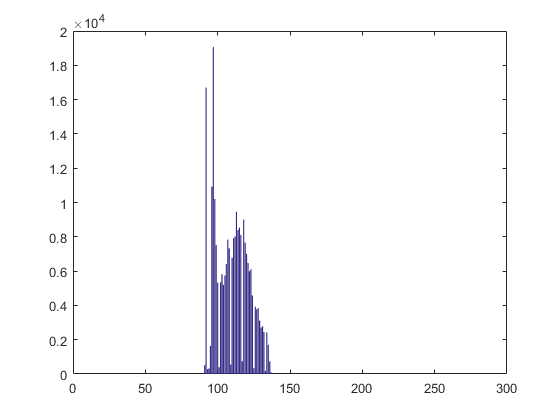
\includegraphics[width=\linewidth]{myfigure/p1/fbar2.png}
    	\caption{}
    	\label{fig:fbar2}
  	\end{subfigure}
	\begin{subfigure}[b]{0.45\linewidth}
    	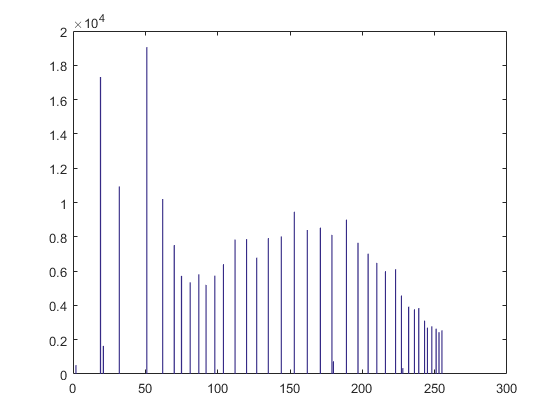
\includegraphics[width=\linewidth]{myfigure/p1/gbar2.png}
    	\caption{}
    	\label{fig:gbar2}
  	\end{subfigure}
  	\caption{Results of Fig2.jpg. (a)Original image. (b)Processed image after applying histogram equalization. (c)Histogram of original image. (d)Histogram of processed image.}
  	\label{fig:result2}
\end{figure}

\clearpage

\subsection{Discussion}
We can see that histograms are quite different from continuous functions because there are gaps between each horizontal value. So the histogram of the equalized image is like a sparse version of the original image. The result of Fig2(low contrast ratio) shows an increasing on contrast ratio and it's more useful than the original result. However, Fig1(high contrast ratio) is not a good example of histogram equalization. The affect is just like a intensity transition. We can simply draw a not so serious conclusion that histogram equalization is useful for images with low contrast ratio but not for images with high contrast ratio.

\subsection{Implementation}
There is some key part of my implementation.
\lstset{language=Matlab}
\begin{lstlisting}
function [x, y] = histShow( imgf )
%HISTSHOW display the histogram graph of the imgf
% x - the horizontal axis of histogram, 
% y - the vertical axis of histogram
g = imgf(:) + 1;
n = length(g);
x = (1 : 256);
y = zeros(1, 256);
for i = (1 : n)
    y(g(i)) = y(g(i)) + 1;
end

end

function [ imgg ] = histEqual( imgf )
%HISTEQUAL 
%   
[x, y] = histShow(imgf);
T = zeros(1, 256);
a = 0;
g = imgf(:);
n = length(g);
for i = (1 : 256)
    T(i) = a + y(i);
    a = T(i);
end
T = round(255 * T / n);
for i = (1 : n)
    g(i) = T(g(i)+1);
end
imgg = reshape(g, size(imgf));

end
\end{lstlisting}





\section{Project 2 - Spatial Enhancement Methods}
\subsection{Project Proposal}
Implement the image spatial enhancement task showed in text book Figure 3.43. The steps involve Laplacian
filter, Sobel filter, average filter and power law transformation.

\subsection{Preliminaries}
\subsubsection{Basic Spatial Filtering}
In general, linear spatial filtering of an image of size $M\times N$ with a filter of size $m \times n$ is \begin{equation} g(x,y)=\sum_{s=-a}^a \sum_{t=-b}^b  w(s,t)f(x+s,y+t) \end{equation} where $a=(m-1)/2$ and $b=(n-1)/2$. There are two closely related concepts related to spatial filtering.
One is \emph{correlation} and the other is \emph{convolution}. Correlation of filter $w(x, y)$ is defined as \begin{equation}\sum_{s=-a}^a \sum_{t=-b}^b  w(s,t)f(x+s,y+t) \end{equation} while convolution is defined as \begin{equation} \sum_{s=-a}^a \sum_{t=-b}^b  w(s,t)f(x-s,y-t) \label{eq:convdefine}\end{equation}
 The confusion point is that we usually call spatial filter as convolution filter, convolution mask or convolution kernel but the terms are not necessarily refer to the true convolution operation defined in Eq.\ref{eq:convdefine}. 

\subsubsection*{Smoothing spatial filters}
Smoothing filters are used for blurring and for noise reduction. The simplest smoothing filter is averaging filters, which is also called lowpass filter. $M \times N$ averaging filter can be represented as \begin{equation} g(x,y)=\frac{\sum_{s=-a}^a \sum_{t=-b}^b w(s,t)f(x+s,y+t)}{\sum_{s=-a}^a \sum_{t=-b}^b w(s,t)} \end{equation} The simple idea of filter size choosing is that choose the approximately the same size of the noisy you want to reduce. Average filter is an example of linear spatial filters. There are also nonlinear order-static spatial filters using the ranking information of each pixel. We will talk about order-static filters in \emph{Project 8}. 

\subsubsection*{Sharpening spatial filters}
The principal objective of sharpening is to highlight transitions in intensity. Because averaging is analogous to integration, it is logical to conclude that sharpening can be accomplished by spatial differentiation. Thus we consider the sharpening filters based on first- and second-order derivatives. \newline
\textbf{Second-order derivatives - the Laplacian} \newline
Laplacian is defined as \begin{equation} \nabla^2 f=\frac{\partial^2f}{\partial x^2}+\frac{\partial^2f}{\partial y^2} \end{equation} In x-direction and y-direction we have \begin{equation} \frac{\partial^2f}{\partial x^2} = f(x+1,y)-f(x,y)-(f(x,y)-f(x-1,y))=f(x+1,y)+f(x-1,y)-2f(x,y) \end{equation} \begin{equation} \frac{\partial^2f}{\partial y^2} = f(x,y+1)-f(x,y)-(f(x,y)-f(x,y-1))=f(x,y+1)+f(x,y-1)-2f(x,y) \end{equation}
Thus we get the discrete Laplacian of two variables:
\begin{equation}
nabla^2 f(x,y)=f(x+1,y)+f(x-1,y)f(x,y+1)+f(x,y-1)-4(x,y)
\label{eq:lapfilter}\end{equation} Based on Eq.\ref{eq:lapfilter} we have 4 masks displayed in Fig.\ref{fig:lapfilter}. The basic way we use Laplacian for image sharpening is \begin{equation} g(x,y)=f(x,y)+c\left[ \nabla^2 f(x,y) \right] \end{equation} where $c=1$ if we use Fig.\ref{fig:lap3} or Fig.\ref{fig:lap4}. 

\begin{figure}[h!]
	\centering
	\begin{subfigure}[b]{0.2\linewidth}
		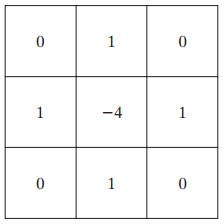
\includegraphics[width=\linewidth]{myfigure/p2/lap-1.png}
		\caption{}
		\label{fig:lap1}
	\end{subfigure}
	\begin{subfigure}[b]{0.2\linewidth}
    	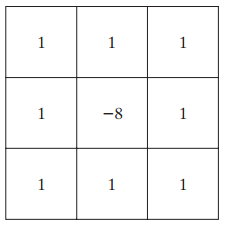
\includegraphics[width=\linewidth]{myfigure/p2/lap-2.png}
		\caption{}
		\label{fig:lap2}
  	\end{subfigure}
  	\begin{subfigure}[b]{0.2\linewidth}
		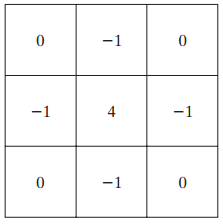
\includegraphics[width=\linewidth]{myfigure/p2/lap-3.png}
		\caption{}
		\label{fig:lap3}
	\end{subfigure}
	\begin{subfigure}[b]{0.2\linewidth}
    	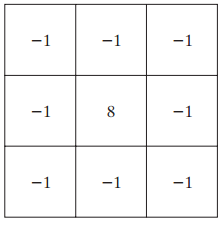
\includegraphics[width=\linewidth]{myfigure/p2/lap-4.png}
		\caption{}
		\label{fig:lap4}
  	\end{subfigure}
  	\caption{4 Laplacian masks. \textbf{(a)}Direct implementation of Eq.\ref{eq:lapfilter}. \textbf{(b)}Extent (a) by adding two diagonal terms. \textbf{(c)(d)} sign inverse of (a)(b) relatively. More common in practice.}
  	\label{fig:lapfilter}
\end{figure}

\textbf{First-order derivatives - the gradient} \newline
First-order derivatives in image processing using the magnitude of the gradient. The gradient vector is \begin{equation} \nabla f \equiv \text{grad}(f) \equiv \left[ \begin{array}{c} g_x \\ g_y \end{array}\right] = \left[ \begin{array}{c} \frac{\partial f}{\partial x} \\ \frac{\partial f}{\partial y} \end{array} \right] 
\end{equation}
The magnitude of vector $\nabla f$ defined as \begin{equation}M(x,y)=mag(\nabla f) =  \sqrt{g_x^2 + g_y^2} \approx |g_x| + |g_y| \end{equation} is the value of the rate of change in the direction of the gradient vector. The second = is a frequently used approximate to avoid square roots. A widely used approximate filter masks implementing gradient is Sobel defined as \begin{equation} g_x = \frac{\partial f}{\partial x} =  (z_7+2z_8+z_9) - (z_1+2z_2+z_3)\end{equation} and \begin{equation} g_y = \frac{\partial f}{\partial y} =  (z_3+2z_6+z_9) - (z_1+4z_2+z_7)\end{equation}
$3\times 3$ Sobel filter is displayed in Fig.\ref{fig:sobel}
\begin{figure}[h!]
	\centering
	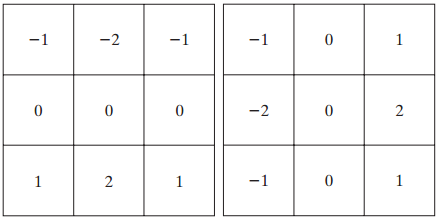
\includegraphics[scale=0.6]{myfigure/p2/sobel.png}
	\caption{$3\times 3$ SObel mask. Left is on x direction, right is on y direction.}
	\label{fig:sobel}
\end{figure}

\subsection{Experiment - Combining Spatial Enhancement}
We conduct the experiment on the Fig.2.3a image of whole body bone scan. Our goal is to enhance this image by sharpening it and by bringing out more of the skeletal detail. The narrow dynamic ranging of the intensity levels and high noise content make this problem difficult. The process and result images are displayed in Fig.\ref{fig:abcd} and Fig.\ref{fig:efgh}. Here, I describe the detail process of the enhancement. \newline
We first use Laplacian with the mask in Fig.\ref{fig:lap4} to extract the sharp transitions in intensity. Note that Fig.2.3b is a scaled result because the numerical matrix result contains negative values which can not be visualized as image by matlab default function. After obtaining Laplacian, we add Laplacian(not the scaled one by the real laplacian) to the original image to get the sharpened Fig.2.3c. This step is just follow Eq.\ref{eq:lapfilter}. In Fig.2.3d we compute the Sobel gradient of original image using masks in Fig.\ref{fig:sobel}. Edges are more dominant than ones in Laplacian. In Fig.2.4e we use $5 \times 5 $averaging filter to smooth the Sobel gradient for noisy reduction purpose. It’s not proper to use median filter because medical image processing requires high level of convince. In Fig.2.4f, we multiply the Laplacian with Sobel. Multiply seems like a strange operation but we can consider it as use Sobel to mask Laplacian in order to strengthen edges and reduce noisy. In Fig.2.4g we sum up the product and the original image. Finally in Fig.2.4h we increase the dynamic range of the sharpened image by powerlaw transformation which is defined as
\begin{equation} s-cr^\gamma \end{equation} where we use $\gamma=0.5$ and $c=1$. We use $\gamma <1$ to spread the intensity level and note that histogram equalization would not give use satisfying result as discussed in Project 1.

\subsection{Discussion}
We finally get a satisfy result in the Fig.2.4h which shows significant new visible features. There are two tricks we should pay attention to. First, the operations may produce intensity levels out of the range $[0,255]$. In this kind of cases, a direct matlab command \emph{imshow()} will cause problem. So we have to use scale function. While coding, I made a mistake that I didn’t take the numerical type into consideration. I gain an experience that before computation, transform the matrix type to double at first.

\subsection{Implementation}
Here I paste the key parts of my matlab implementation.
\lstset{language=Matlab}
\begin{lstlisting}
function [ imgg ] = replicate_padding( imgf, pad )
%REPLIACTE_PADDING
% imgf - img to be padded, pad - amount of padding 
[M, N] = size(imgf);
% repmat(mat, row_rep, col_rep);
top = repmat(imgf(1, :), pad, 1);
button = repmat(imgf(M, :), pad, 1);
left = repmat(imgf(:, 1), 1, pad);
right = repmat(imgf(:, N), 1, pad);
lt = repmat(imgf(1,1), pad, pad);
rt = repmat(imgf(1,N), pad, pad);
lb = repmat(imgf(M,1), pad, pad);
rb = repmat(imgf(M,N), pad, pad);
imgg = [lt, top, rt; left, imgf, right; lb, button, rb];
end
\end{lstlisting}

\lstset{language=Matlab}
\begin{lstlisting}
function [ scale_imgg, imgg] = b_laplacian_scale( imgf )
%B_LAPLACIAN_SCALE 
[M, N] = size(imgf);
% padding
f = replicate_padding(imgf, 2);
f = double(f);
% laplacian
mask = [-1 -1 -1; -1 8 -1; -1 -1 -1];
g = zeros(M+4, N+4);
for x = (2 : M+3)
    for y = (2 : N+3)
        g(x, y) = sum(sum(f(x-1:x+1, y-1:y+1) .* mask));
    end
end
imgg = g(3:M+2, 3:N+2); % laplacian result without scale
% scale
scale_imgg = scale255(imgg);
end
\end{lstlisting}
\lstset{language=Matlab}
\begin{lstlisting}
function [ imgg ] = d_sobel( imgf )
%D_SOBEL 
[M, N] = size(imgf);
f = replicate_padding(imgf, 2);
f = double(f); % double f
% Sobel
maskx = [-1 -2 -1; 0 0 0; 1 2 1];
masky = [-1 0 1; -2 0 2; -1 0 1];
gx = zeros(M+4, N+4);
gy = zeros(M+4, N+4);
for x = (2 : M+3)
    for y = (2 : N+3)
        gx(x, y) = sum(sum(f(x-1:x+1, y-1:y+1) .* maskx));
        gy(x, y) = sum(sum(f(x-1:x+1, y-1:y+1) .* masky));
    end
end
% new image: using abs
gx = abs(gx(3:M+2, 3:N+2));
gy = abs(gy(3:M+2, 3:N+2));
imgg = scale255(gx+gy);
end
\end{lstlisting}
\lstset{language=Matlab}
\begin{lstlisting}
function [ imgg ] = scale255( imgf )
%SCALE255 
% return is uint8 type
%imgf = double(imgf);
[M, N] = size(imgf);
K = 255;

minf = zeros(M, N) + min(min(imgf));
maxf = zeros(M, N) + max(max(imgf));
imgg = K * (imgf-minf) ./ (maxf - minf);
imgg = uint8(imgg);
end
\end{lstlisting}

\lstset{language=Matlab}
\begin{lstlisting}
function [ imgg ] = e_5x5_average( imgf )
%E_5X5_AVERAGE
[M, N] = size(imgf);
% padding
f = replicate_padding(imgf, 4);
f = double(f);
% 5x5 average
g = zeros(M+8, N+8);
for x = (3 : M+6)
    for y = (3 : N+6)
        g(x, y) = sum(sum(f(x-2:x+2, y-2:y+2))) / 25;
    end
end
imgg = g(5:M+4, 5:N+4); % laplacian result without scale
imgg = uint8(imgg);
end
\end{lstlisting}

\clearpage

\begin{figure}[h!]
	\centering
	\begin{subfigure}[b]{0.4\linewidth}
		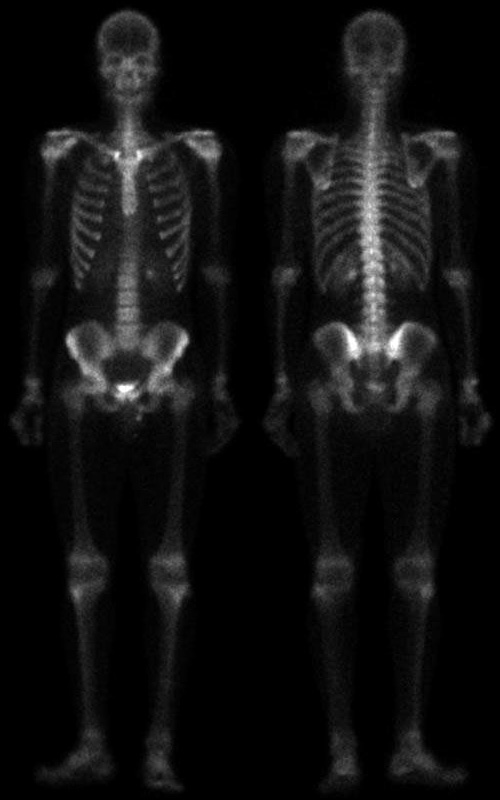
\includegraphics[width=\linewidth]{myfigure/p2/2-a.png}
		\caption*{(a)}
		\label{fig:2a}
	\end{subfigure}
	\begin{subfigure}[b]{0.4\linewidth}
    	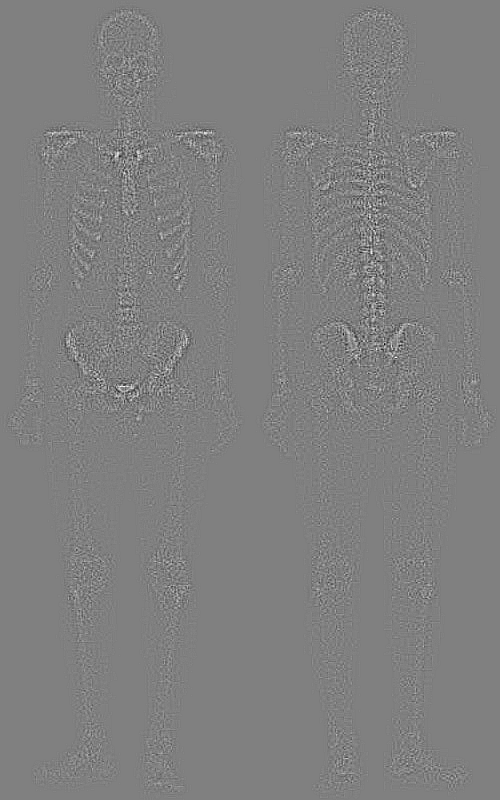
\includegraphics[width=\linewidth]{myfigure/p2/2-b.png}
		\caption*{(b)}
		\label{fig:2b}
  	\end{subfigure}
  	\begin{subfigure}[b]{0.4\linewidth}
		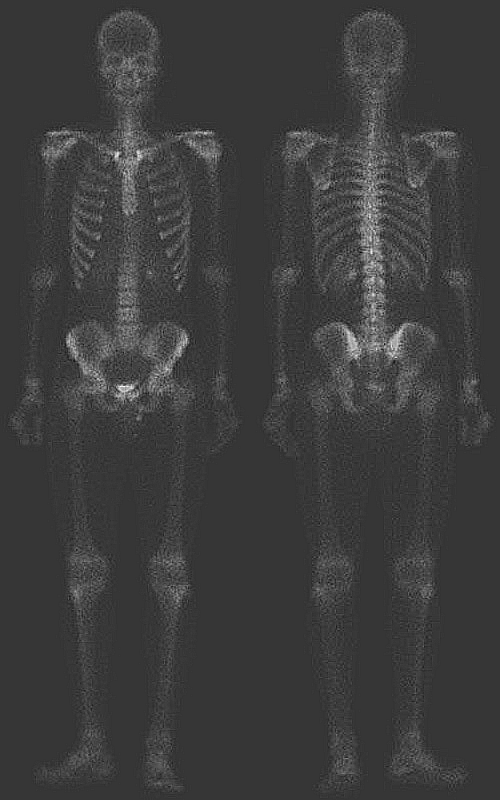
\includegraphics[width=\linewidth]{myfigure/p2/2-c.png}
		\caption*{(c)}
		\label{fig:2c}
	\end{subfigure}
	\begin{subfigure}[b]{0.4\linewidth}
    	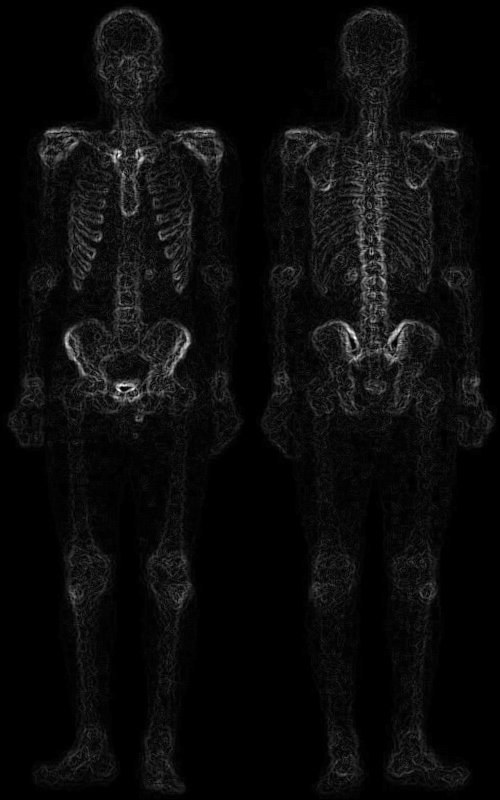
\includegraphics[width=\linewidth]{myfigure/p2/2-d.png}
		\caption*{(d)}
		\label{fig:2d}
  	\end{subfigure}
  	\caption{\textbf{a}Original image of whole body bone scan. \textbf{(b)}Laplacian of (a)(Rescaled to [0,255]). \textbf{(c)}Sharpened image obtained by add (a) and (c). \textbf{(d)}Sobel gradient of (a).}
  	\label{fig:abcd}
\end{figure}
\clearpage
\begin{figure}[h!]
	\centering
	\begin{subfigure}[b]{0.4\linewidth}
		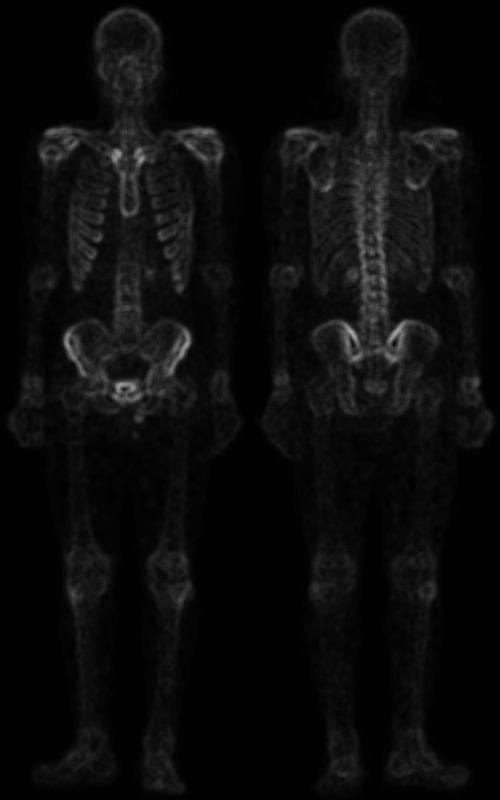
\includegraphics[width=\linewidth]{myfigure/p2/2-e.png}
		\caption*{(e)}
		\label{fig:2e}
	\end{subfigure}
	\begin{subfigure}[b]{0.4\linewidth}
    	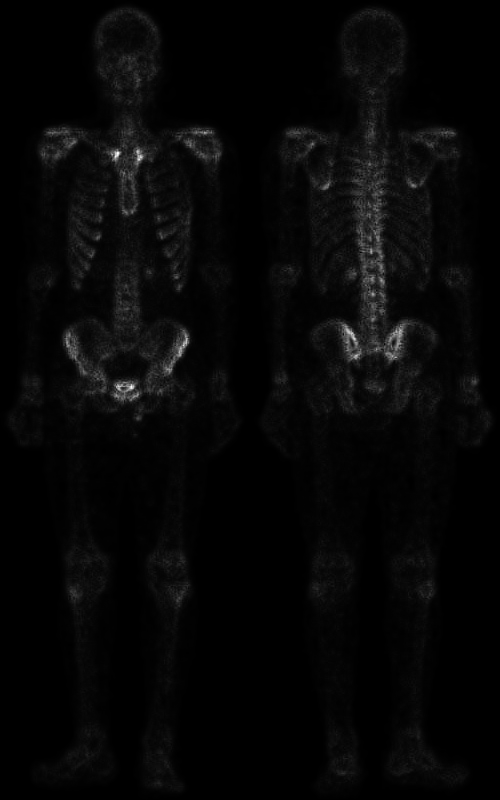
\includegraphics[width=\linewidth]{myfigure/p2/2-f.png}
		\caption*{(f)}
		\label{fig:2f}
  	\end{subfigure}
  	\begin{subfigure}[b]{0.4\linewidth}
		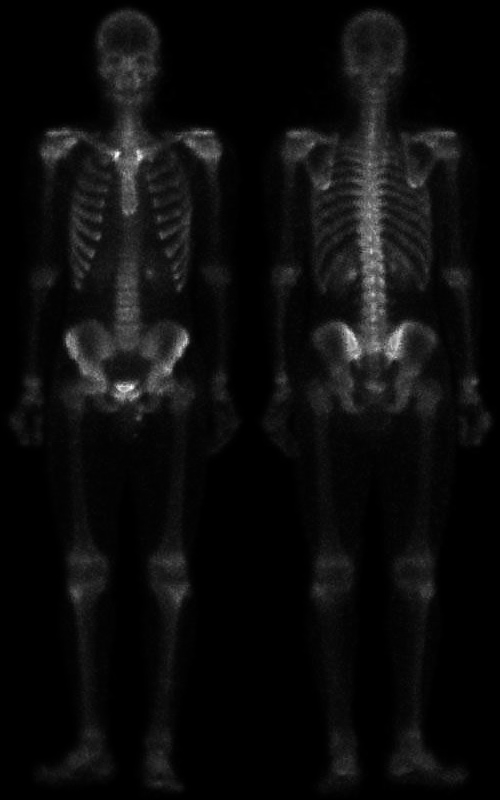
\includegraphics[width=\linewidth]{myfigure/p2/2-g.png}
		\caption*{(g)}
		\label{fig:2g}
	\end{subfigure}
	\begin{subfigure}[b]{0.4\linewidth}
    	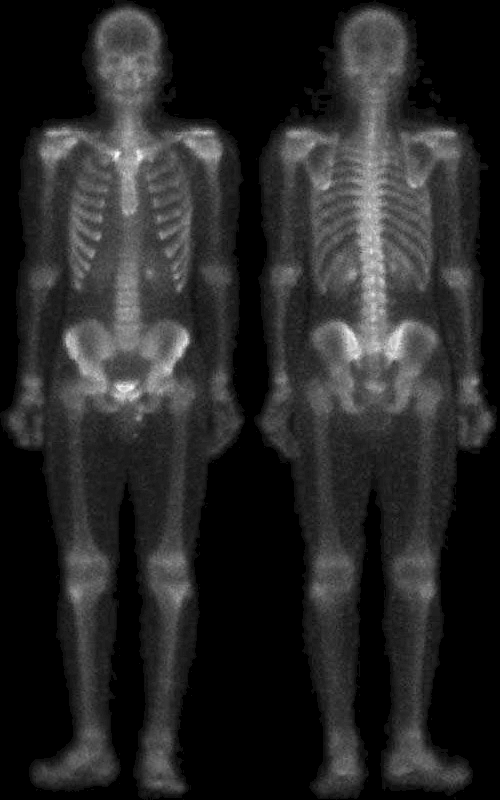
\includegraphics[width=\linewidth]{myfigure/p2/2-h.png}
		\caption*{(h)}
		\label{fig:2h}
  	\end{subfigure}
  	\caption{\textbf{(e)}Sobel image smoothed with $5\times 5$ averaging filter. \textbf{(f)}Mask image formed by the product of (c) and (e). \textbf{(g)}Sharpened image obtained by applying a power-law transformation to (g). \textbf{(h)}Compare (g) and (h).}
  	\label{fig:efgh}
\end{figure}



\section{Project 3 - Filtering in Frequency Domain}

\subsection{Project Proposal}
Implement the ideal, Butterworth and Gaussian lowpass and highpass filters and the results under different parameters using the image character\_test\_pattern.tif

\subsection{Preliminaries}
\subsubsection{Summary of Fourier transform properties}

\begin{table}[h]
	\caption{Summary of useful formulas.}
	\centering
	\begin{tabular}{|l|m{0.6\columnwidth}|}\hline
		Name & Expression(s) \\ \hline
		1D FT & \begin{equation}F(u)=\int_{-\infty}^\infty f(t)e^{-j2 \pi ut}dt \end{equation} \\ 
		1D IFT & \begin{equation}f(t)=\int_{-\infty}^\infty F(u)e^{j2 \pi ut}du\end{equation} \\
		1D DFT & \begin{equation}F(u)=\sum_{t=0}^{M-1}f(t)e^{-j2\pi ut/M} \end{equation} \\
		1D IDFT & \begin{equation}f(t)=\frac{1}{M}\sum_{u=0}^{M-1}F(u)e^{j2\pi ut/M}\end{equation} \\
		2D FT & \begin{equation} F(u,v)=\int_{-\infty}^\infty \int_{-\infty}^\infty f(x,y)e^{-j2 \pi (ux+vy)}dxdy \end{equation} \\
		2D DFT & \begin{equation} F(u,v)= \sum_{x=0}^{M-1}\sum_{y=0}^{N-1} f(x,y)e^{-j2\pi (ux/M+vy/N)}\end{equation} \\
		2D IDFT & \begin{equation} f(x,y) = \frac{1}{MN}\sum_{u=0}^{M-1}\sum_{v=0}^{N-1]}F(u,v)e^{j2\pi(ux/M+vy/N)} \end{equation} \\
		Power spectrum & \begin{equation} P(u,v)=|F(u,v)|^2 \end{equation} \\
		\hline
	\end{tabular}
\end{table}

\subsubsection{Steps for filtering in the frequency domain}
\begin{enumerate}
	\item Given an input image $f(x,y)$ of size $M\times N$, obtain the padding parameters $P=2M$ and $Q=2N$.Form a padded image, $f_p(x,y)$, of size $P\times Q$ by appending zeros.
	\item Multiply $f_p(x,y)$ by $(-1)^{x+y}$ to center its transform.
	\item Compute the DFT, $F(u,v)$ of the image from centered padded image.
	\item Generate a real, symmetric filter function $H(u,v)$ of size $P \times Q$ with center at coordinates $(P/2, Q/2)$. Form the product $G(u,v)=H(u,v)F(u,v)$.
	\item Obtain the precessed image: $g_p(x,y)=\left\{ \text{real}\left[\ \mathcal{F}^{-1}[G(u,v)] \right] \right\}(-1)^{x+y}$ where the real part is selected in order to ignore parasitic complex components resulting from computational inaccuracies.
	\item Obtain the final processed result, $g(x,y)$, by extracting the top left $M\times N$ quadrant of $g_p(x,y)$
\end{enumerate}


\subsection{Image Smoothing Using Frequency Domain Filters}
Edges and other sharp intensity transitions such as noise in an image contribute significantly to the high-frequency content of its Fourier transform. Hence, smoothing is achieved in the frequency domain by high-frequency attenuation.
\subsubsection{Ideal lowpass filters}
\emph{Ideal lowpass filters (ILPF)} is very sharp as it is specified by the function 
\begin{equation}
H(u,v) = \left \{ \begin{array}{rcl}
1 & \text{if $D(u,v)\leq D_0$} \\
0 & \text{otherwise}
\end{array} \right.
\end{equation}
where $D_0$ is a positive constant and $D(u,v)$ is the distance between  $(u,v)$ in frequency domain and the center of the frequency rectangle; that is \begin{equation} D(u,v) = \left[ (u-P/2)^2+(v-Q/2)^2 \right]^{1/2} \end{equation} 
One way to establish a set of standard cutoff frequency loci is to compute circles that enclose specified amounts of total image power $P_T$. \begin{equation} P_T=\sum_{u=0}^{P-1}\sum_{v=0}^{Q-1}P(u,v) \end{equation}
The percentage of power enclosed by the circle of radius $D_0$ with origin at the center of the frequency rectangle is \begin{equation} \alpha=100\left[\ \sum_u\sum_vP(u,v)/P_T \right] ~~~~ \text{(u,v) is inside the circle}\end{equation}

\section{Project 4 - Image Restoration}
\subsection{Project Proposal}
First implement the random noise generation functions. The random noise functions include uniform, Gaussian, Rayleigh, Gamma, exponential and impulse. Requirement is that only uniform noise is allowed to use built-in function while any other noise should be generated based on uniform noise with self-defined functions. The test image is \emph{Fig0503.tif}.
Second follow the process shown in textbook \emph{FIGURE 5.7, FIGURE 5.8, FIGURE 5.10, FIGURE 5.11, FIGURE 5.12}. Each figure displays a process of add some specified type of noise and then use restoration method to reduce noise.

\subsection{Preliminaries}
\subsubsection{Noise Models}
The principal source of noise in digital images arise during image acquisition and/or transmission. We assume in this project that noise is independent of spatial coordinates and uncorrelated with respect to the image itself. Thus, what we concerned is the statistical behavior of the intensity value in the noise component which can be described by PDF. 

We can view the random variable from another view that does not involved PDF directly by generating random variable from uniform distribution. The idea is similar to the one we use in project 1's histogram equalization. 




\section{Project 6 - Geometric Transformation}
\subsection{Project Proposal}


\section{Project 8 - Morphological Processing}

\subsection{Project Proposal}
Implement the \emph{"Opening by reconstruction", "Filling holes" and "Border clearing"} operations on textbook \emph{chapter 9.5}. The task is to reproduce the results in \emph{Figure 9.29, 9.31 and 9.32}.

\subsection{Preliminaries}
\subsubsection{Basic morphological operations}
Morphology offers a unified and powerful approach to numerous image processing problem. These operations defined based on set theory. In this project we consider that morphological operations are conducted on binary images (preprocessing is required for gray-level images). The below table describes the basic widely used morphological processing.
\begin{table}[h]
	\caption{Summary of basic morphological operations.}
	\centering
	\begin{tabular}{|l|l|m{0.45\columnwidth}|}\hline
		Operation & Equation & Comments\\ \hline
		Translation & $(B)_z=\{w|w=b+z, ~ b \in B \}$ & Translation the origin of $B$ to point $z$.\\
		Reflection & $\hat{B}=\{w|w=-b, ~ b \in B\}$ & Reflects all elements of B about the origin of this set.\\
		Complement & $A^c=\{ w|w \notin A \}$ & Set of points not in $A$.\\
		Difference & $A-B=\{ w|w \in A, w \notin B\}$ & Set of points that belong to $A$ but not to $B$.\\
		Dilation & $A \oplus B=\left\{ z|(\hat{B}_z) \cap A \neq \emptyset \right\}$ & Expands the boundary of $A$.\\
		Erosion & $A \ominus B=\left\{ z|(B)_z \subseteq A \right\}$ & Contracts the boundary of $A$.\\
		Opening & $A \circ B=(A\ominus B)\oplus B $ & Smoothes contours, breaks narrow isthmuses, and eliminates small islands and sharp peaks.\\
		Closing & $A \bullet B=(A\oplus B)\ominus B $ & Smoothes contours, fuses narrow breaks and long thin gulfs and eliminates small holes.\\
		Hit-or-miss transform & $A \otimes B=(A\ominus B_1)\cap(A^c\ominus B_2)$ & The set of pints at which, simultaneously $B_1$ found a hit in $A$ and $B_2$ found a match in $A^c$.\\ \hline
	\end{tabular}
\end{table}

\subsubsection{Morphological restoration}
With the basic operations, we can discuss a powerful morphological transformation \emph{morphological restoration} that involves two images and a structuring element. One image, the \emph{marker}, contains the starting points for the transformation. The other image, the \emph{mask}, constrains the transformation. \\
\subsubsection*{Geodesic dilation and erosion}
Geodesic dilation and erosion are the central concepts to morphologic reconstruction. Let $F$ denote the maker and $G$ denote the mask and $F \subseteq G$. The \emph{geodesic dilation} of size 1 of the marker with respect to the mask, denoted by $D_G^(1)(F)$, is defined as 
\begin{equation} D_G^{(1)}(F)=(F\oplus B) \cap G \end{equation}
The geodesic dilation of size $n$ of $F$ with resplect to $G$ is defined as 
\begin{equation} D_G^{(n)}(F)=D_G^{(1)} \left[ D_G^{(n-1)}(F) \right]\end{equation}
with $D_G^{(0)}(F)=F$. Similarly, the \emph{geodesic erosion} of size 1 of marker $F$ with respect to mask $G$ is defined as 
\begin{equation} E_G^{(1)}(F)=(F\ominus B) \cup G \end{equation}
The geodesic erosion of size $n$ of $F$ with respect to $G$ is defined as
\begin{equation} E_G^{(n)}(F)=E_G^{(1)} \left[ E_G^{(n-1)}(F) \right]\end{equation}
with $E_G^{(0)}(F)=F$. Geodesic dilation and erosion are duals with respect to set complementation. \\
\subsubsection*{Morphological reconstruction by dilation and by erosion}
\emph{Morphological reconstruction by dilation of a mask $G$ from a marker $F$}, denoted $R_G^D{F}$ is defined \begin{equation}R_G^D(F)=D_G^{(k)}(F)\end{equation} with $k$ such that \begin{equation}D_G^{(k)}(F)=D_G^{(k+1)}(F)\end{equation} \emph{Morphological reconstruction by erosion of mask $G$ from a marker $F$}, denoted $R_G^E(F)$ is defined \begin{equation}R_G^E(F)=E_G^{(k)}(F)\end{equation} with $k$ such that \begin{equation}E_G^{(k)}(F)=E_G^{(k+1)}(F)\end{equation}


\subsection{Task-1 Opening by reconstruction}
The opening by reconstruction of size $n$ of an image $F$ is defined as the reconstruction by dilation of $F$ from the erosion of size $n$ of $F$; that is \begin{equation}O_R^{(n)}(F)=R_F^D \left[ (F\ominus nB) \right]\end{equation} where $(F\ominus nB)$ indicates $n$ erosions of $F$ by $B$. \\
Figure \ref{fig:0929a} is the original image for this task. We are interested in extracting the characters that contain long, vertical strokes. The origin image is of size $918 \times 2018$ pixels. The approximate average height of the tall characters is 50 pixels. Thus we use a structuring element of size $51 \times 1$ pixels to erode the original image. The erosion image is shown in Figure \ref{fig:0929b}. For comparison, Figure \ref{fig:0929c} shows the opening of Figure \ref{fig:0929a} with the same structuring element. Using erosion image (b) as the marker and the original image (a) as mask, we restored the characters containing long vertical strokes accurately via opening by reconstruction. This result is displayed in Figure \ref{fig:0929d}. \\

\begin{figure}[h!]
	\centering
	\begin{subfigure}[b]{0.45\linewidth}
		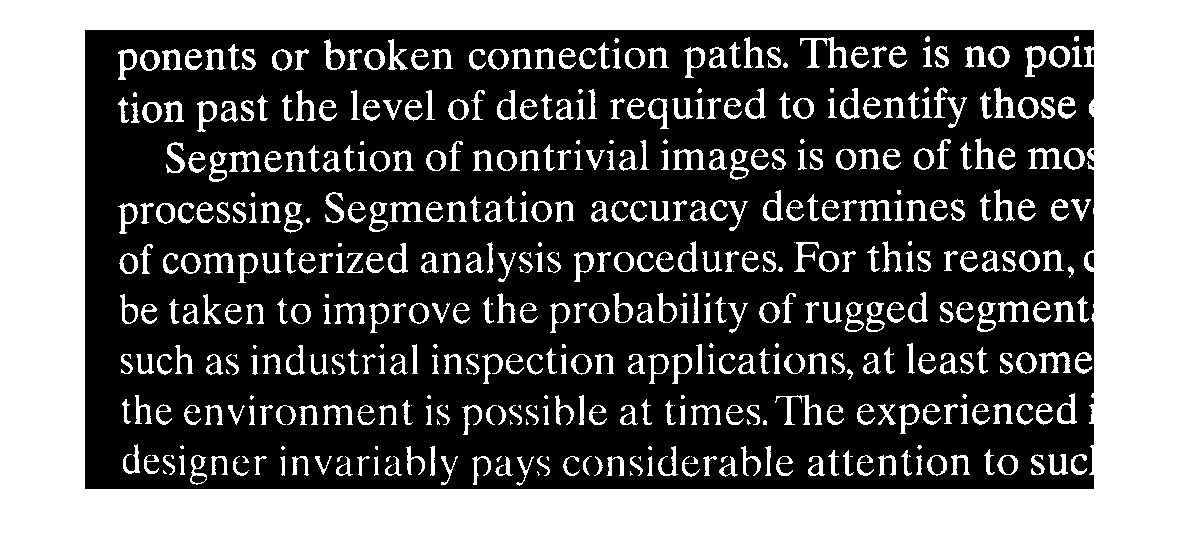
\includegraphics[width=\linewidth]{myfigure/p8/fig0929(a).png}
		\caption{}
		\label{fig:0929a}
	\end{subfigure}
	\begin{subfigure}[b]{0.45\linewidth}
    	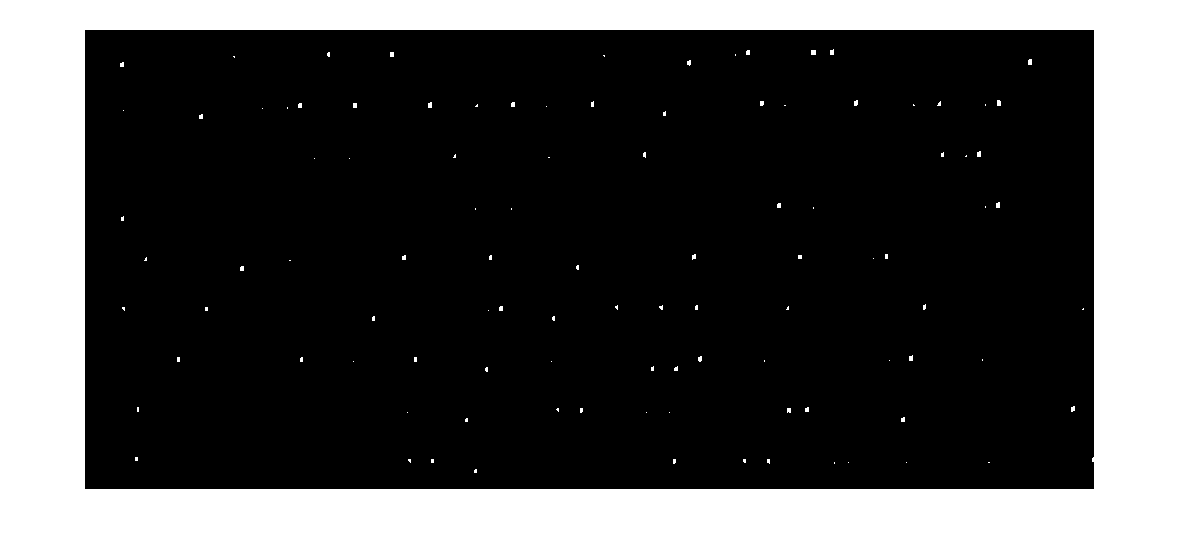
\includegraphics[width=\linewidth]{myfigure/p8/fig0929(b).png}
    	\caption{}
    	\label{fig:0929b}
  	\end{subfigure}
  	\begin{subfigure}[b]{0.45\linewidth}
		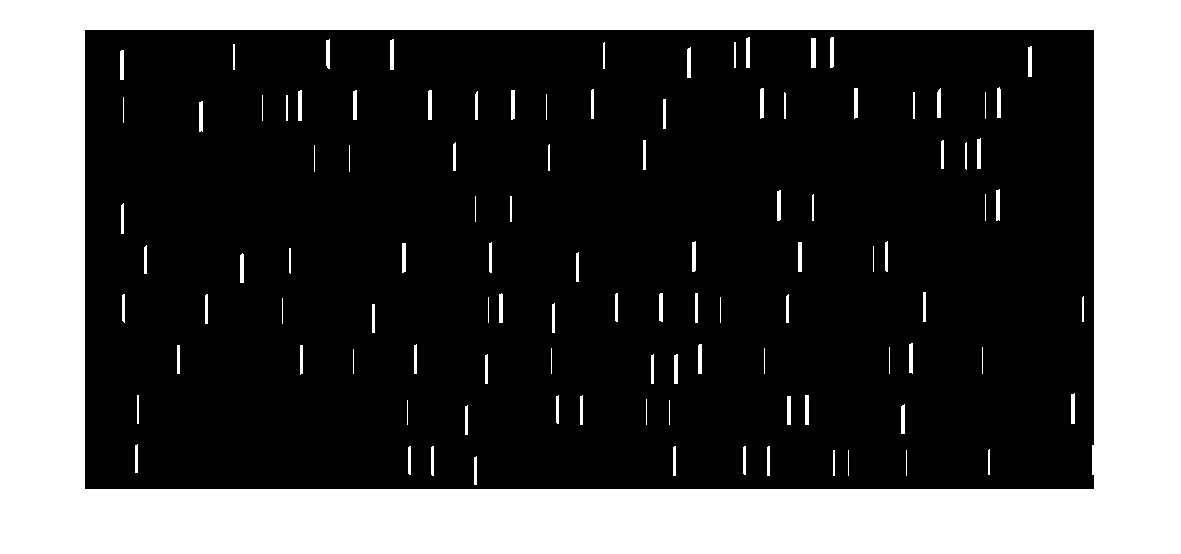
\includegraphics[width=\linewidth]{myfigure/p8/fig0929(c).png}
		\caption{}
		\label{fig:0929c}
	\end{subfigure}
	\begin{subfigure}[b]{0.45\linewidth}
    	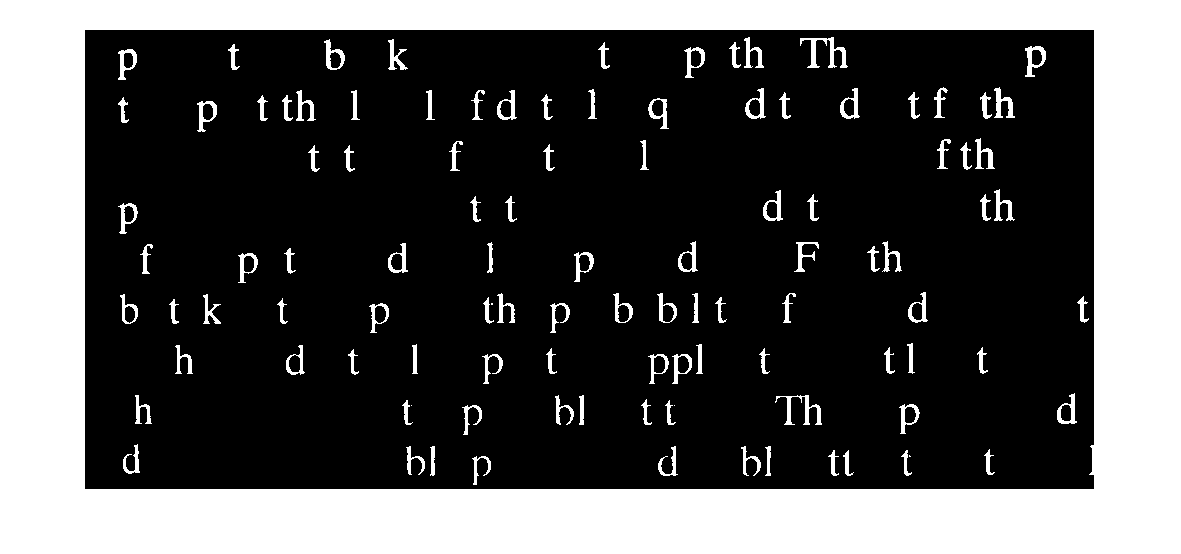
\includegraphics[width=\linewidth]{myfigure/p8/fig0929(d).png}
    	\caption{}
    	\label{fig:0929d}
  	\end{subfigure}
  	\caption{Task1-opening by reconstruction. (a)Original binary image $918 \times 2018$. (b)Erosion of (a) with a structuring element of size $51 \times 1$ pixels. (c)Opening of(a) with the structuring element $51 \times 1$, shown for comparison. (d)Result of opening by reconstruction.}
  	\label{fig:0929}
\end{figure}

The size of geodesic dilation reconstruction is $76$. This process cost about $7$ minutes. I output some of the intermediate results in Figure \ref{fig:0929append} that help us understand the reconstruction better.
\begin{figure}
	\centering
	\begin{subfigure}[b]{0.45\linewidth}
		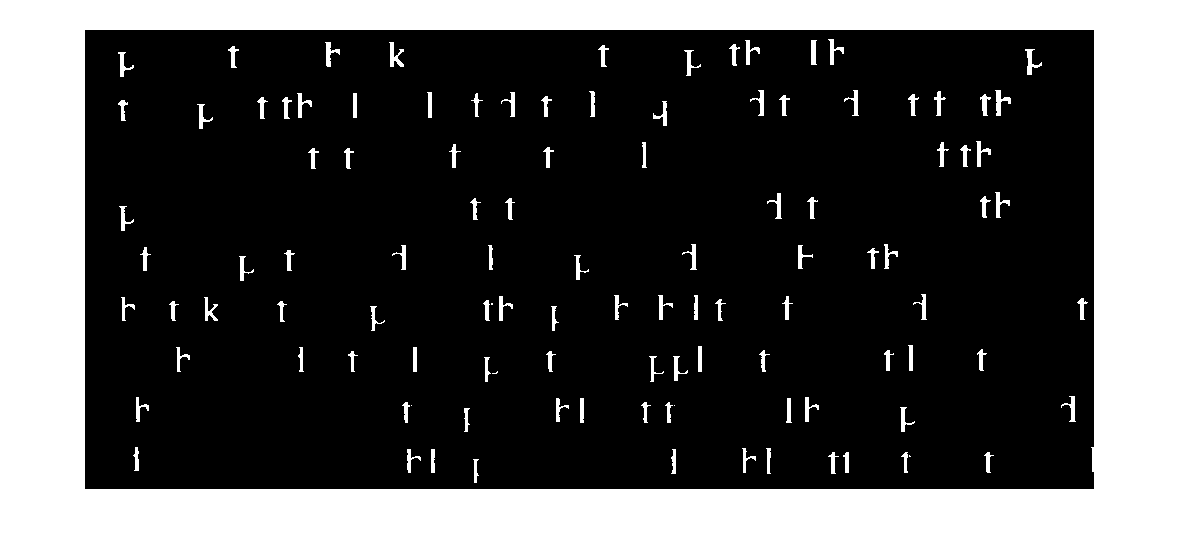
\includegraphics[width=\linewidth]{myfigure/p8/fig0929(d20).png}
		\caption{}
		\label{fig:0929d20}
	\end{subfigure}
	\begin{subfigure}[b]{0.45\linewidth}
    	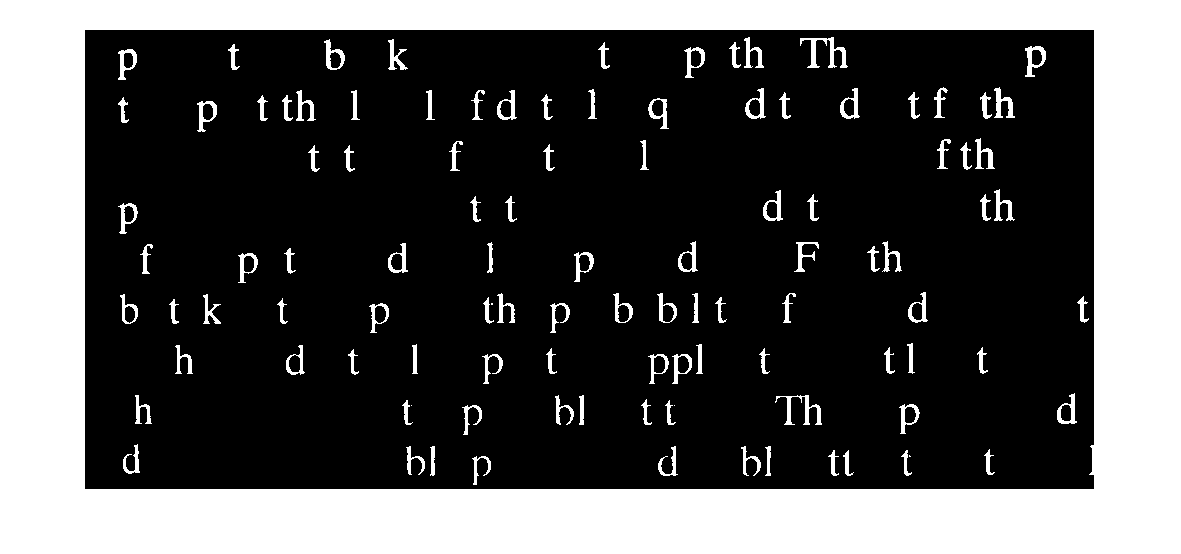
\includegraphics[width=\linewidth]{myfigure/p8/fig0929(d).png}
    	\caption{}
    	\label{fig:0929d76}
  	\end{subfigure}
	\caption{See task-1's process in details. (a)Dilation of size $20$. (b)Dilation of size $76$, the final results.}
  	\label{fig:0929append}
\end{figure}


\subsection{Task-2 Hole filling}
Here we develop a fully automated procedure based on morphological reconstruction. Let $I(x,y)$ denote a binary image and we form a marker $F$ that is $0$ everywhere, except at the image border; that is,
\begin{equation}
F(x, y)=\left\{
\begin{array}{rcl}
1-I(x,y) & \text{if $(x,y)$ is on the border of $I$} \\
0 & \text{otherwise} 
\end{array} \right.
\end{equation}
Then \begin{equation} H=\left[ R_{I^c}^D(F) \right]^c \end{equation} is a binary image equal to $I$ with all holes filled. \\
I use $3\time 3$ structuring element. The hole filling images are shown in Figure \ref{fig:0931}. A detailed process of dilation reconstruction with intermediate results are shown in Figure \ref{fig:0931append}. The reconstruction takes $479$ steps of dilation, which costs a very long period of about $40$ minutes. 
\begin{figure}[h!]
	\centering
	\begin{subfigure}[b]{0.45\linewidth}
		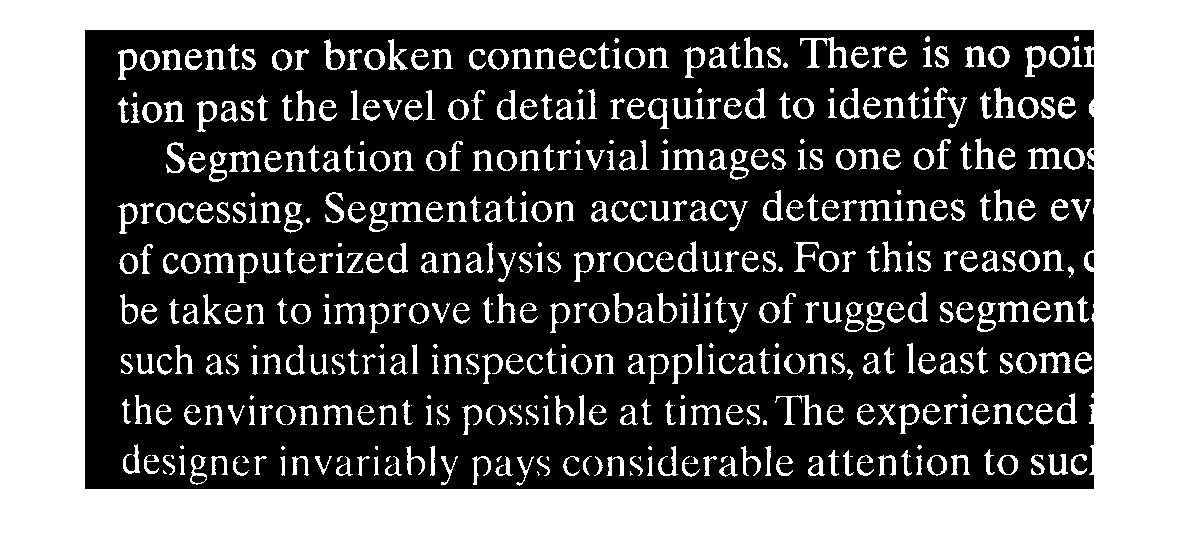
\includegraphics[width=\linewidth]{myfigure/p8/fig0929(a).png}
		\caption{}
		\label{fig:0931a}
	\end{subfigure}
	\begin{subfigure}[b]{0.45\linewidth}
    	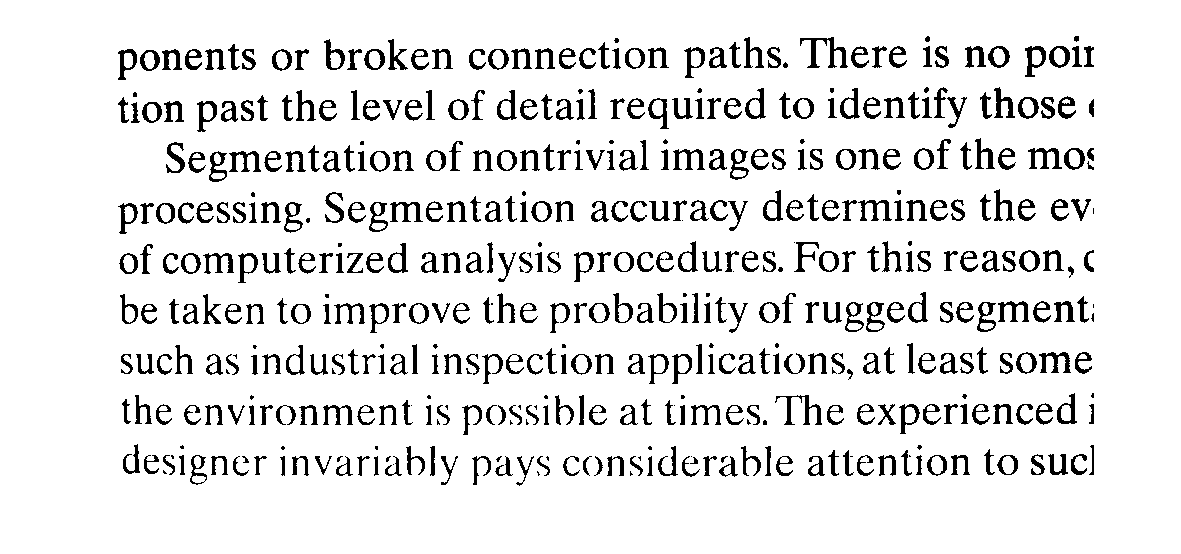
\includegraphics[width=\linewidth]{myfigure/p8/fig0931(b).png}
    	\caption{}
    	\label{fig:0931b}
  	\end{subfigure}
  	\begin{subfigure}[b]{0.45\linewidth}
		
\includegraphics[width=\linewidth]{myfigure/p8/fig0931(c).png}
		\caption{}
		\label{fig:0931c}
	\end{subfigure}
	\begin{subfigure}[b]{0.45\linewidth}
    	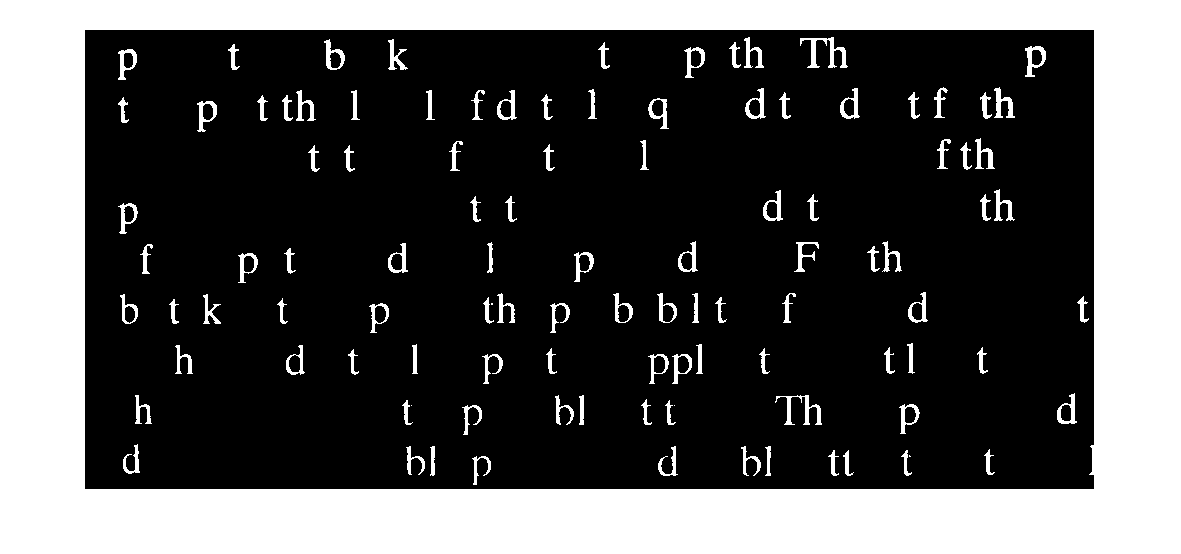
\includegraphics[width=\linewidth]{myfigure/p8/fig0929(d).png}
    	\caption{}
    	\label{fig:0931d}
  	\end{subfigure}
  	\caption{Task2-hole filling. (a)Original binary image $918 \times 2018$. (b)Complement of (a). Used as a mask. (c)Marker image. Seems like a whole black one, but in fact with some white on border. (d)Result of opening by reconstruction.}
  	\label{fig:0931}
\end{figure}

\begin{figure}[h!]
	\centering
	\begin{subfigure}[b]{0.45\linewidth}
		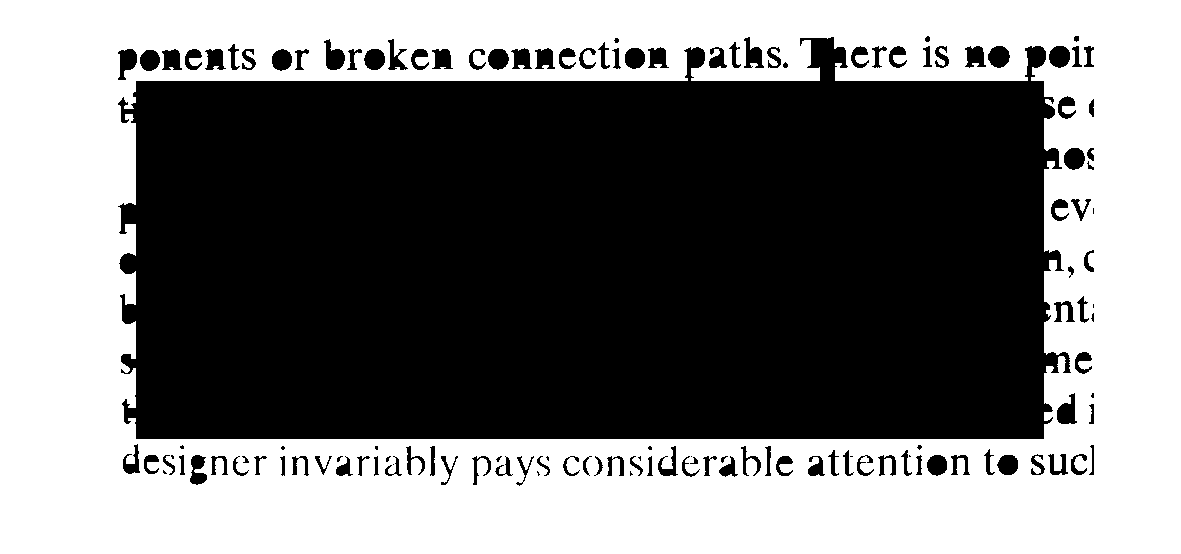
\includegraphics[width=\linewidth]{myfigure/p8/fig0931(d100).png}
		\caption{}
		\label{fig:0931d100}
	\end{subfigure}
	\begin{subfigure}[b]{0.45\linewidth}
    	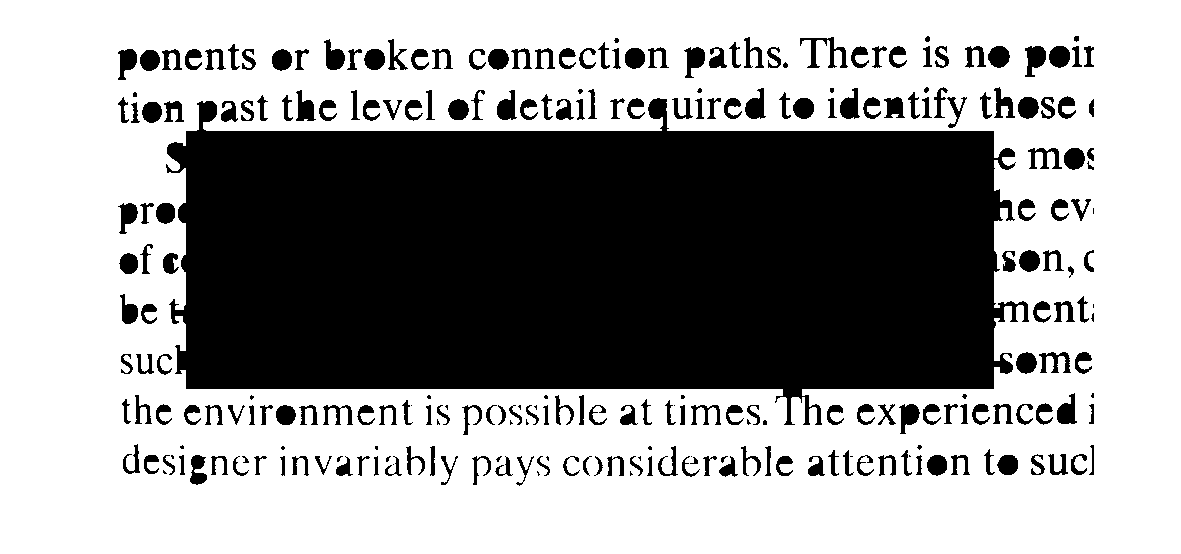
\includegraphics[width=\linewidth]{myfigure/p8/fig0931(d200).png}
    	\caption{}
    	\label{fig:0931d200}
  	\end{subfigure}
  	\begin{subfigure}[b]{0.45\linewidth}
		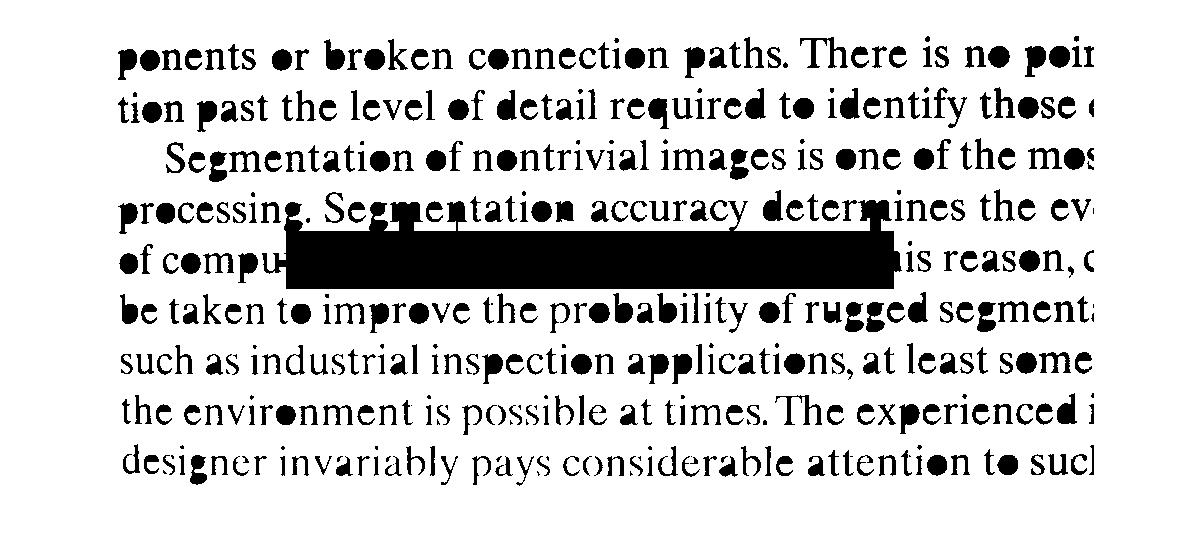
\includegraphics[width=\linewidth]{myfigure/p8/fig0931(d400).png}
		\caption{}
		\label{fig:0931d400}
	\end{subfigure}
	\begin{subfigure}[b]{0.45\linewidth}
    	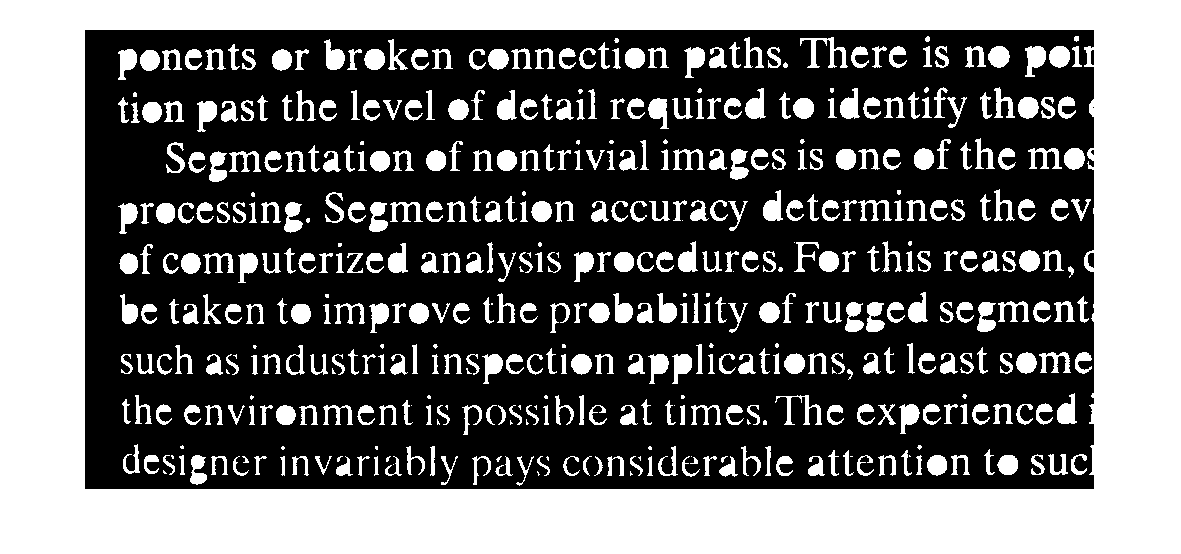
\includegraphics[width=\linewidth]{myfigure/p8/fig0931(d).png}
    	\caption{}
    	\label{fig:0931d479}
  	\end{subfigure}
  	\caption{The process of hole filling in details. (a)After 100 steps of dilation. (b)After 200 steps of dilation. (c)After 400 steps of dilation. Much closer to success! (d)The final result with completion.}
  	\label{fig:0931append}
\end{figure}


\subsection{Task-3 Border clearing}
Removing objects that touch the border is a useful work because it can screen images so that only complete objects remain for further processing. The marker $F(x,y)$ is defined as:
\begin{equation}  
F(x, y)=\left\{
\begin{array}{rcl}
I(x,y) & \text{if $(x,y)$ is on the border of $I$} \\
0 & \text{otherwise} \\
\end{array} \right.
\end{equation}
First we computes morphological reconstruction $R_I^D(F)$ and then computes the desired image $X$
\begin{equation} X=I-R_I^D(F) \end{equation}
I use structuring element of size $3 \times 3$. This task is much easier than task 2 and takes just $21$ steps of dilation in about $2$ minutes. Results are shown in Figure \ref{fig:0932}.
\begin{figure}[h!]
	\centering
  	\begin{subfigure}[b]{0.45\linewidth}
		
\includegraphics[width=\linewidth]{myfigure/p8/fig0932(a).png}
		\caption{}
		\label{fig:0932a}
	\end{subfigure}
	\begin{subfigure}[b]{0.45\linewidth}
    	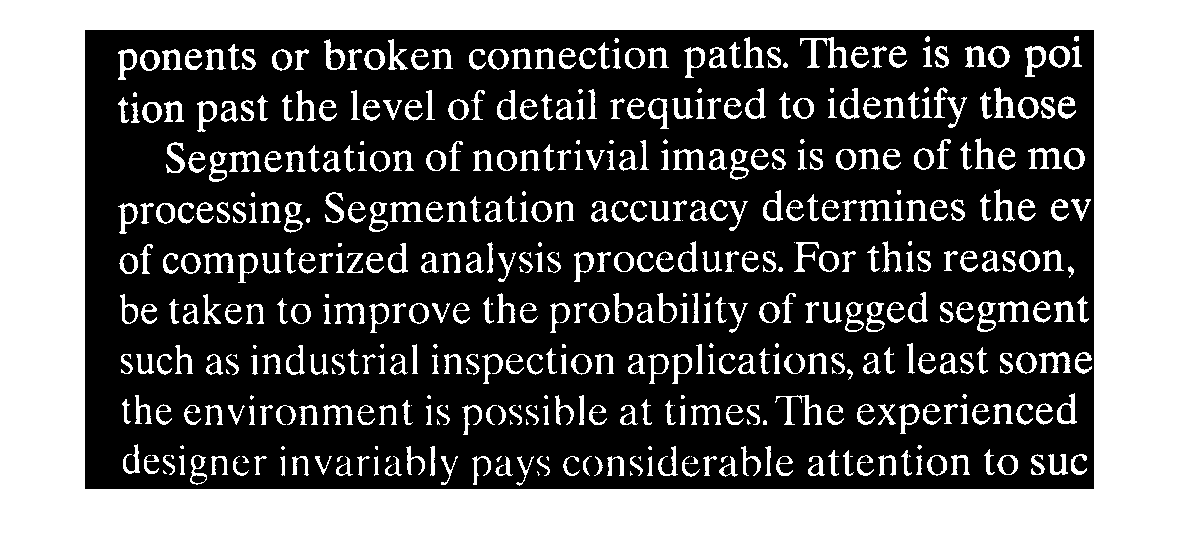
\includegraphics[width=\linewidth]{myfigure/p8/fig0932(b).png}
    	\caption{}
    	\label{fig:0932b}
  	\end{subfigure}
  	\caption{Border clearing. (a)After use border marker for 21-dilation reconstruction. The border letter. (b)The final result after subtraction.}
  	\label{fig:0932}
\end{figure}

\subsection{Implementation}
Matlab functions \emph{erosion, dilation, geodesic\_dilation, dilation\_reconstruction and opening\_reconstruction} are implemented for this project. I made a \textbf{mistake} on opening\_reconstruction at first that I still use $51 \times 1$ as the maker while calling dilation\_reconstruction. The wrong output image is the same as (c) as all the shorter horizontal adjacent relationship in our wanted characters was damaged. So for correction, we must use $3 \times 3$ as structuring element for dilation\_reconstruction called in opening\_reconstruction. \\
In the below code frame, I list the key part of these functions. Other process of calling these functions in main script are trivial so omitted here.\\
\lstset{language=Matlab}
\begin{lstlisting}
% key part of function erosion
for i = (1:M-m+1)
    for j = (1:N-n+1)
        x = imgf(i:i+m-1, j:j+n-1);
        if sum(sum(x.*B)) == m*n
            g(i+downshift, j+rightshift) = 1;
        end
    end
end

% key part of dilation_reconstruction 
k_times = 0;
while( ~isequal(f0, f1) )
    k_times = k_times + 1;
    f0 = f1;
    f1 = geodesic_dilation(f1, G, B);
end

% key part of geodesic_dilation
imgg = dilation(imgf, B) & G;

% key part of opening_reconstruction
for i=(1:n_size)
    f_erosion = erosion(f_erosion, B);
end
[imgg, k_times] = dilation_reconstruction(f_erosion, imgf, ones(3,3)); % here can not use ones(51, 1)
\end{lstlisting}

\subsection{Discussion}
These three tasks show the basic idea of morphological reconstruction used in feature extraction. We start from a marker which can be  obtained easily. Then we use the mask as the constrain to conduct set operations. More advanced topics are morphological operations on gray intensity images and image segmentation. This is a very interesting subproject.
The main obstacle here is \textbf{time}! I tried to do much vectorization but still have a big problem that 20-step-dilation cost about 2 minutes on the $918\times 2018$ image but the complexity is only about $918 \times 2018 \times 20 \times 9 \approx 4 \times 10^8$. I think the computation of this complexity need no more than 2 sec on language like C++ or python. However, I tried the matlab toolbox \emph{IPT} and it's just as fast as the expectation (within 2 sec). This is a strange but interesting problem.

\section{Project 9 - Image Segmentation}

\subsection{Project Proposal}
There tow parts of project 9. One task is for edge detection: implement the Roberts, Prewitt, Sobel, the Marr-Hildreth and the Canny edge detectors. The test image is \emph{building.tif}. The other task is to implement the Otsu’s method of thresholding segmentation, and compare the results with the global thresholding method using test image \emph{polymersomes.tif}.

\subsection{Preliminaries}
\subsubsection{Edge detection}
The central idea of edge detection is that local changes in intensity can be detected using derivatives. We have the following conclusions which show that first- and second-order derivatives are particularly well suited for this purpose: (1) First-order derivatives generally produce thicker edges in an image. (2) Second-order derivatives have a stronger response to fine details such as thin lines, isolated points, and noise. (3) Second-order derivatives produce a double-edge response at ramp and step transitions in intensity. (4) The sign of the second derivative can be used to determine whether a transition into an edge is from light to dark or dark to light.

\subsubsection{Basic edge detection}
The tool of choice for finding edge strength and direction at location $(x, y)$ of an image $f$ is the gradient. 
\begin{equation} \nabla f \equiv \text{grad}(f) \equiv \left[ \begin{array}{c} g_x \\ g_y \end{array}\right] = \left[ \begin{array}{c} \frac{\partial f}{\partial x} \\ \frac{\partial f}{\partial y} \end{array} \right] 
\end{equation}
The magnitude of vector $\nabla f$ defined as \begin{equation} \label{eq:magnitude} M(x,y)=mag(\nabla f) =  \sqrt{g_x^2 + g_y^2} \approx |g_x| + |g_y| \end{equation} is the value of the rate of change in the direction of the gradient vector. The second $=$ is a frequently used approximate to avoid square roots. The direction of gradient vector is given by the angle \begin{equation} \alpha(x,y)=\tan^{-1} \left[ \frac{g_y}{g_x} \right] \label{eq:angle} \end{equation}
The direction of an edge at an arbitrary point $(x,y)$ is orthogonal to the direction $\alpha(x,y)$. 
Here we mention three masks(Figure \ref{fig:3masks}) Roberts, Prewitt and Sobel which can be used to compute the gradient of the center point with convolution operation.
\begin{figure}[h!]
	\centering
	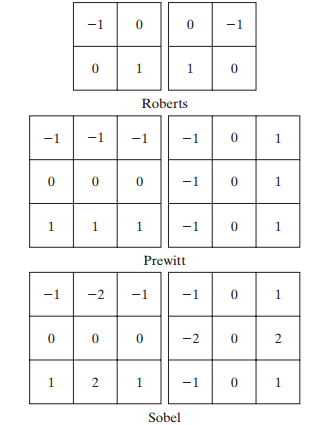
\includegraphics[scale=0.7]{myfigure/p9/3masks.png}
	\caption{3 masks for gradient computation: Roberts, Prewitt, Sobel}
	\label{fig:3masks}
\end{figure}

\subsubsection{More advanced techniques for edge detection}
\textbf{The Marr-Hildreth edge detector} is able to compute the approximate numerical result of gradient operator for sharply focused detail as well as act at large scale to detect the blurry edges. This operator is defined as $\nabla^2 G$ where \begin{equation}G(x,y) = e^{-frac{x^2+y^2}{2\sigma^2}} \label{eq:gaussian_2}\end{equation}. Then the so-called \emph{Laplacian of Gaussian(LoG)} is \begin{equation} \nabla^2 G(x,y) = \left[ \frac{x^2+y^2-\sigma^2}{4\sigma^4} \right]e^{-\frac{x^2+y^2}{2\sigma^2}} \end{equation} The use of LoG filter can be represented as \begin{equation} g(x,y)=\nabla^2\left[G(x,y)\right]\circ f(x,y) \end{equation}. Because of linear process, we can also write it as \begin{equation} g(x,y)=\nabla^2\left[G(x,y)\circ f(x,y)\right] \end{equation} 
Hence, the steps of Marr-Hildreth algorithm can be summarized as: \textbf{1.}Filter the input image with $n\times n$ Gaussian lowpass filter obtained by sampling \ref{eq:gaussian_2}. \textbf{2.}Compute the Laplacian of the result of step \textbf{1} using, for example, $3\times 3$ mask. \textbf{3.}Find the zero crossing of the resulting image from step 2. \\
The method of finding zero crossing at any pixel $p$ is to use a $3\times 3$ neighborhood centered at $p$, if the absolute difference of any two opposite neighbors exceeds a given threshold, then $p$ is a zero-crossing pixel.\\
\\
\textbf{The Canny edge detector} is superior in general to all the detectors discussed before. The algorithm consist the following steps: \\
\textbf{1.}Smooth the input image with a Gaussian filter.\\ 
\textbf{2.}Compute the gradient magnitude $M(x,y)$ and angle $\alpha(x,y)$ images. \\
\textbf{3.}Apply nonmaxima suppression to the gradient magnitude image. \\
\textbf{4.}Use double thresholding and connectivity analysis to detect and link edge. \\
The first two steps are apparent as the definition in Eq.\ref{eq:magnitude} and Eq.\ref{eq:angle}. The step \textbf{3 nonmaxima suppression} is used to thin the coarse edges in magnitude image. The essence of nonmaxima suppression is to define a set of discrete orientation of the edge normal $\{ d_1, d_2, d_3, d_4 \}$, e.g. $0^\circ$, $45^\circ$, $90^\circ$, $-45^\circ$. To map edges of arbitrary direction to the discrete orientation, we define non-overlapping range for each given direction. We can formulate the nonmaxima suppression schema for a $3\times 3$ region centered at every point $(x,y)$ in angle image $\alpha(x,y)$: \\
\textbf{(1)}Find the direction $d_k$ that is closest to $\alpha(x,y)$. \\
\textbf{(2)}If the value of $M(x,y)$ is less than at least one of its two neighbor on this direction, let $g_N(x,y)=0$; otherwise, let $g_N(x,y)=M(x,y)$. \\
Then we come to step \textbf{4 double thresholding} on $g_N(x,y)$ to reduce the false edge points. In Canny's algorithm we use two thresholds, $T_L$ as the low threshold and $T_H$ as the high threshold. Canny suggests that the ratio of the high to low threshold should be two or three to one. The process of thresholding is, \begin{equation} g_{NH}(x,y)=g_N(x,y)\geq T_H \end{equation}\begin{equation} g_{NL}(x,y)=g_N(x,y)\geq T_L\end{equation} then eliminate all the nonzero pixels in $g_{NH}$ from $g_{NL}$ \begin{equation} g_{NL}(x,y) := g_{NL}(x,y)-g_{NH}(x,y) \end{equation} The pixels in $g_{NH}$ is viewed as strong valid edge pixels and are marked immediately, but there are many gaps on these edges that should be filled using information from $g_{NL}$. We do this by following these steps:\\
\textbf{(1)}Locate the next unvisited edge pixel $p$ in $g_{NH}$. \\
\textbf{(2)}Mark all the weak pixels in $g_{NL}$ that is 8-connective to $p$ as valid. \\
\textbf{(3)}If all nonzero pixels in $g_{NH}$ has been visited, goto step 4. Otherwise goto back to step 1. \\
\textbf{(4)}Set all the pixels that are not marked as valid in $g_{NL}$.\\
The final result of Canny's algorithm is formed by appending all the nonzero pixels in $g_{NL}$ to $g_{NH}$.
\subsubsection{Thresholding Segmentation}
Thresholding is useful in applications of image segmentation because of its simplicity of implementation and computational speed. We talk about the most basic intensity thresholding here. The basic formula is 
\begin{equation}g(x,y)=\left \{ \begin{array}{rcl}
1 & \text{if}f(x,y)>T \\
0 & \text{otherwise}  \end{array} \right.\label{eq:global_threshold}\end{equation}
When $T$ is a constant applicable over an entire image, the process given in this equation is referred to as \textbf{global thresholding}. \\
\\
\textbf{Basic global thresholding} algorithm is capable of estimate automatically the threshold value for each image is required. The following iterative algorithm can be used for this purpose:\\
\textbf{1.}Select an initial estimate for the global threshold $T$. Mean value of gray intensities is a good choice.\\
\textbf{2.}Segment the image using $T$ in Eq.\ref{eq:global_threshold}. This will result in two groups of pixels: $G_1$($g(x,y)>T$) and $G_2$($g(x,y)\leq T$)\\
\textbf{3.}Compute the average intensity values $m_1$ and $m_2$ for the two groups $G_1$ and $G_2$ respectively.\\
\textbf{4.}Compute a new threshold value: $T=(m_1+m_2)/2$\\
\textbf{5.}Repeat step2 through 4 until the difference between values of $T$ in successive iterations os smaller than a predefined parameter $\Delta T$.\\
Global thresholding seems very simple as we just need to select a proper value for $T$, but the problem is that, usually, we cannot directly find out such a $T$ that separates the hills in histogram. Noise in the image, illumination and reflectance and so on factors lead to this effect.
Then we discuss an attractive alternative \textbf{Otus's method} which is based entirely on computations performed on the histogram of an image. The algorithm can be summarized as follows:\\
\textbf{1.} Compute the normalized histogram of the input image. Denote the components of the histogram by $p_i, i=0,1,...,L-1$.\\
\textbf{2.} Compute the cumulative sums, $P_1(k)$, for $k=0,1,...,L-1$, using \begin{equation} P_1(k)=\sum_{i=0}^k p_i \end{equation}
\textbf{3.} Compute the cumulative means, $m(k)$, for $k=0,1,...,L-1$ using \begin{equation} m(k)=\sum_{i=0}^k ip_i\end{equation}
\textbf{4.} Compute the global intensity mean, $m_G$, using \begin{equation} m_G=\sum_{i=0}^{L-1}ip_i \end{equation}
\textbf{5.} Compute the between-class variance, $\sigma^2_B(k)$, for $k=0,1,...,L-1$ using \begin{equation} \sigma_B^2(k)=\frac{[m_GP_1(k)-m(k)]^2}{P_1(k)[1-P_1(k)]}\end{equation}
\textbf{6.} Obtain the Otsu threshold, $K^*$, as the value of $k$ for which $\sigma_B^2(k)$ is maximum. If the maximum is not unique, obtain $k^*$ by averaging the values of $k$ corresponding to the various maxima detected. \\
\textbf{7.} Obtain the separability measure, $\eta ^ *$, by at $k=k^*$ evaluating \begin{equation} \eta(k)=\frac{\sigma_B^2(k)}{\sigma_G^2}, \sigma_G^2=\sum_{i=0}^{L-1}(i-m_G)^2p_i \end{equation} 

\subsection{Experiment}
\subsubsection{Edge detection}
First, I display the basic method that only use derivative mask for convolution. These masks are \emph{Roberts, Prewitt and Sobel}. The results are shown in Fig.\ref{fig:basic_edge}. We can see that the result of Sobel and Prewitt is very similar while the result of Roberts is not as good as the two because of lower significance of edges.\\

\begin{figure}[h!]
	\centering
	\begin{subfigure}[b]{0.45\linewidth}
		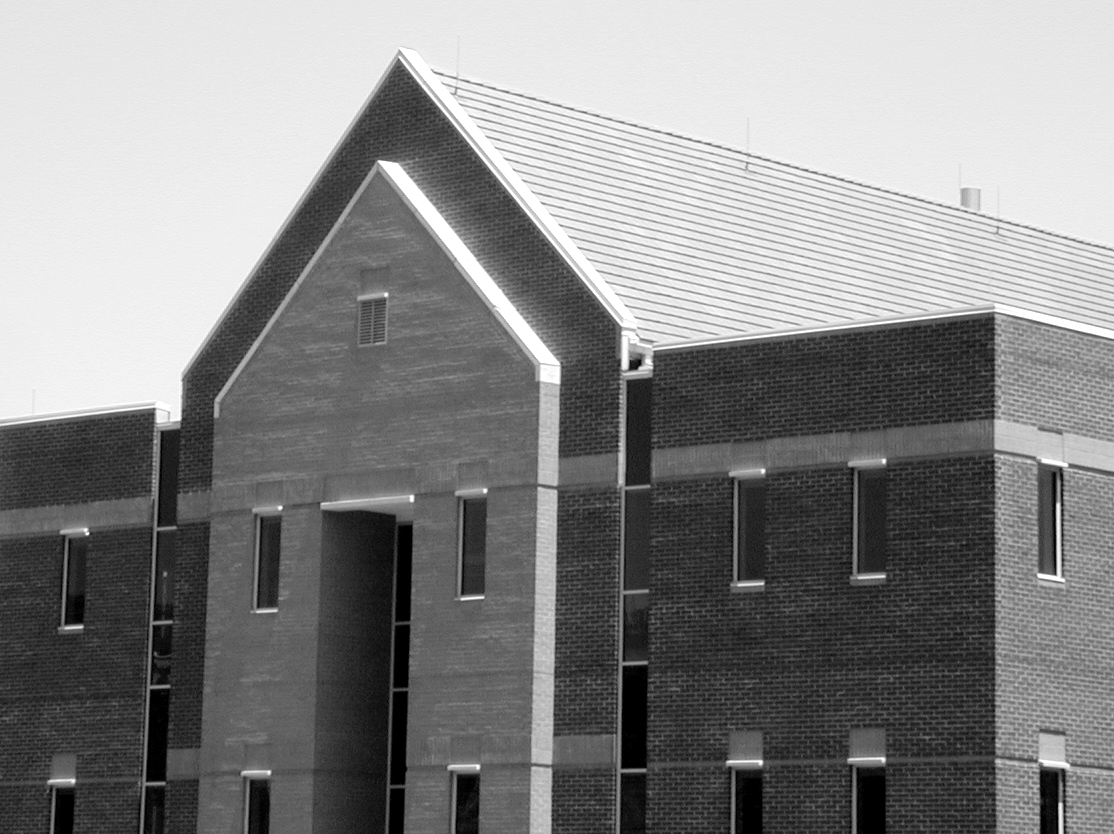
\includegraphics[width=\linewidth]{myfigure/p9/building.png}
		\caption{}
		\label{fig:basic_building}
	\end{subfigure}
	\begin{subfigure}[b]{0.45\linewidth}
    	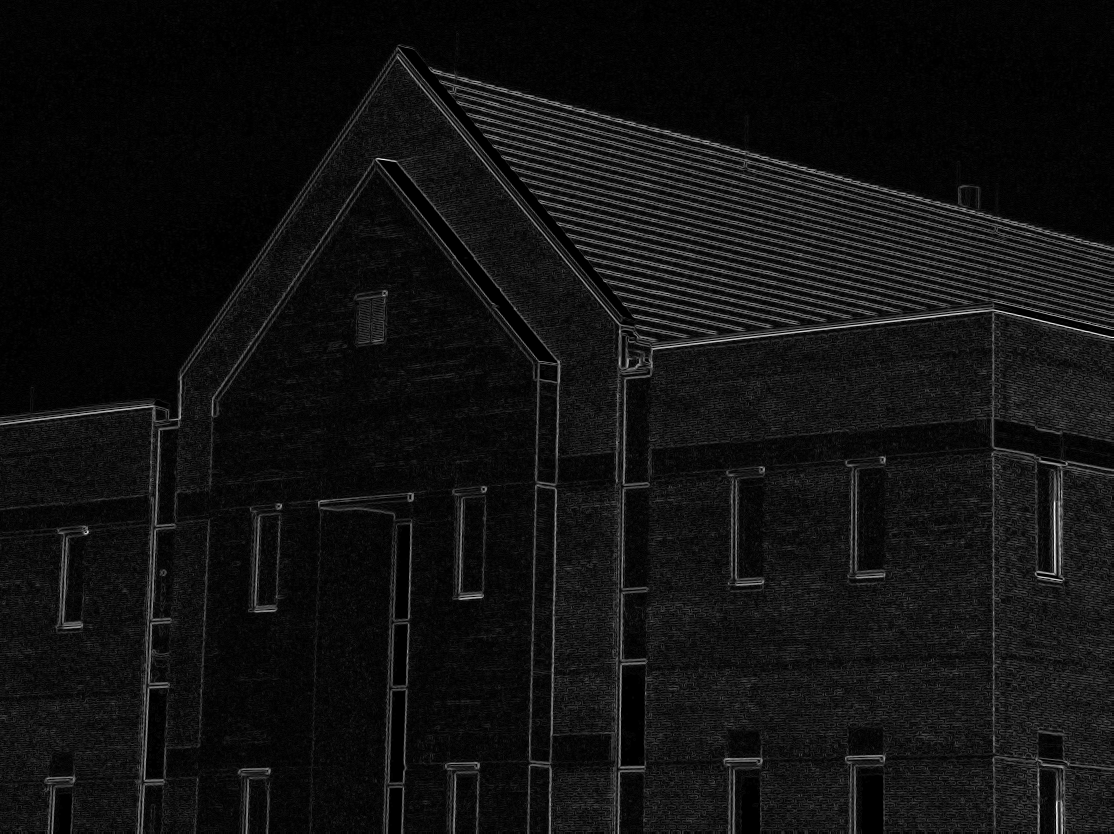
\includegraphics[width=\linewidth]{myfigure/p9/9_roberts.png}
    	\caption{}
    	\label{fig:roberts}
  	\end{subfigure}
  	\begin{subfigure}[b]{0.45\linewidth}
		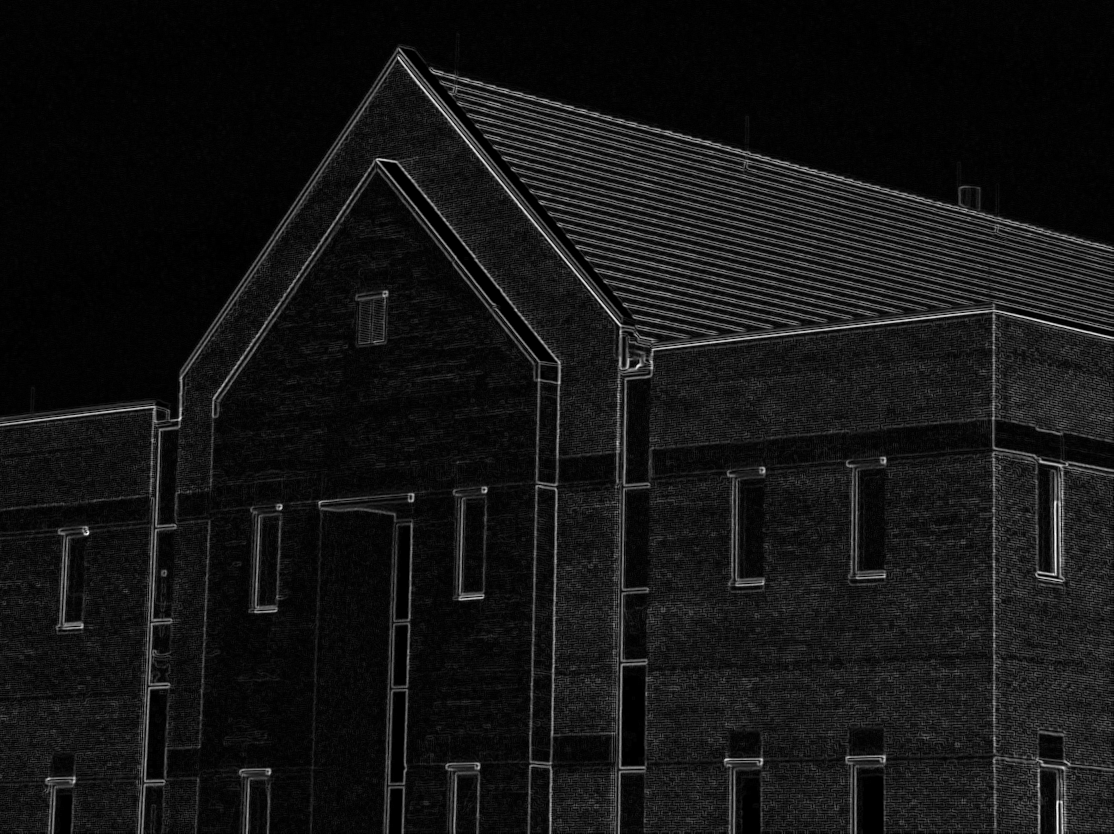
\includegraphics[width=\linewidth]{myfigure/p9/9_prewitt.png}
		\caption{}
		\label{fig:prewitt}
	\end{subfigure}
	\begin{subfigure}[b]{0.45\linewidth}
    	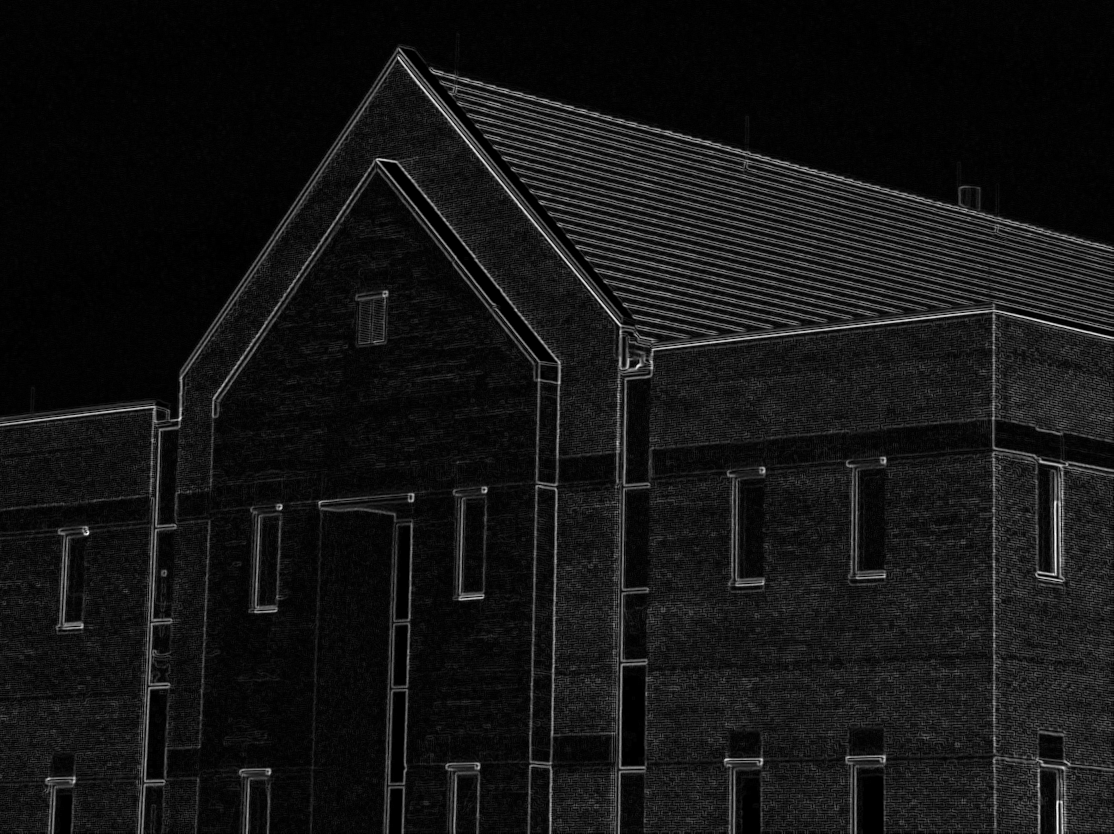
\includegraphics[width=\linewidth]{myfigure/p9/9_sobel.png}
    	\caption{}
    	\label{fig:sobel}
  	\end{subfigure}
  	\caption{Basic edge detection methods. (a)Original test image of size $834 \times 1115$. (b)Edge detection by Roberts mask. (c) Edge detection by Prewitt mask. (d)Edge detection by Sobel mask.}
  	\label{fig:basic_edge}
\end{figure}

Second, I show the process of applying Marr-Hildreth algorithm in Fig.\ref{fig:marr_hildreth}. In (c)-(d), we can see the effect of using threshold. I think that the use of Gaussian lowpass filter is a good idea for create margin between edge and other pixels. As there may be some trivial different between builtin function and self-defined function, the parameters used here is different from the ones given on the textbook. The size of Gaussian lowpass filter is $25\times 25$ and the variance is $\sigma=4$. After trying threshold as 0.04, 0.08, 0.12, I find $0.08$ is the best one.\\

\begin{figure}[h!]
	\centering
	\begin{subfigure}[b]{0.45\linewidth}
		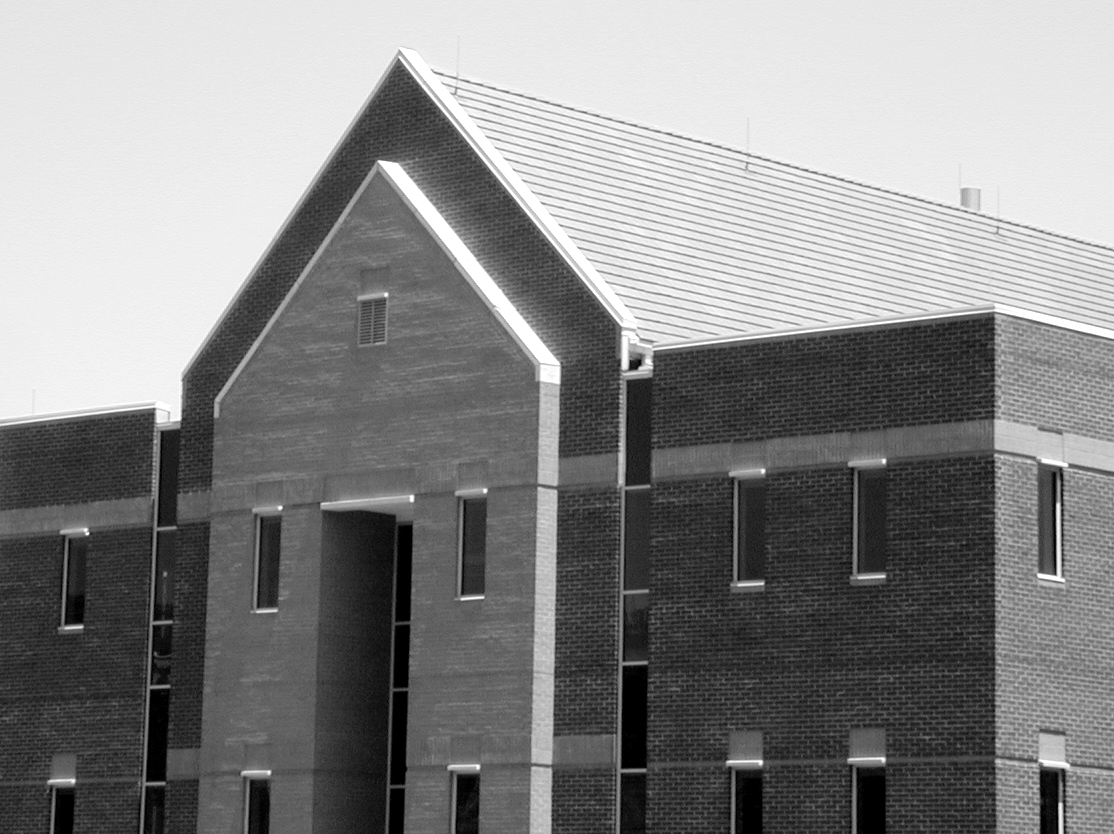
\includegraphics[width=\linewidth]{myfigure/p9/building.png}
		\caption{}
		\label{fig:marr_building}
	\end{subfigure}
	\begin{subfigure}[b]{0.45\linewidth}
    	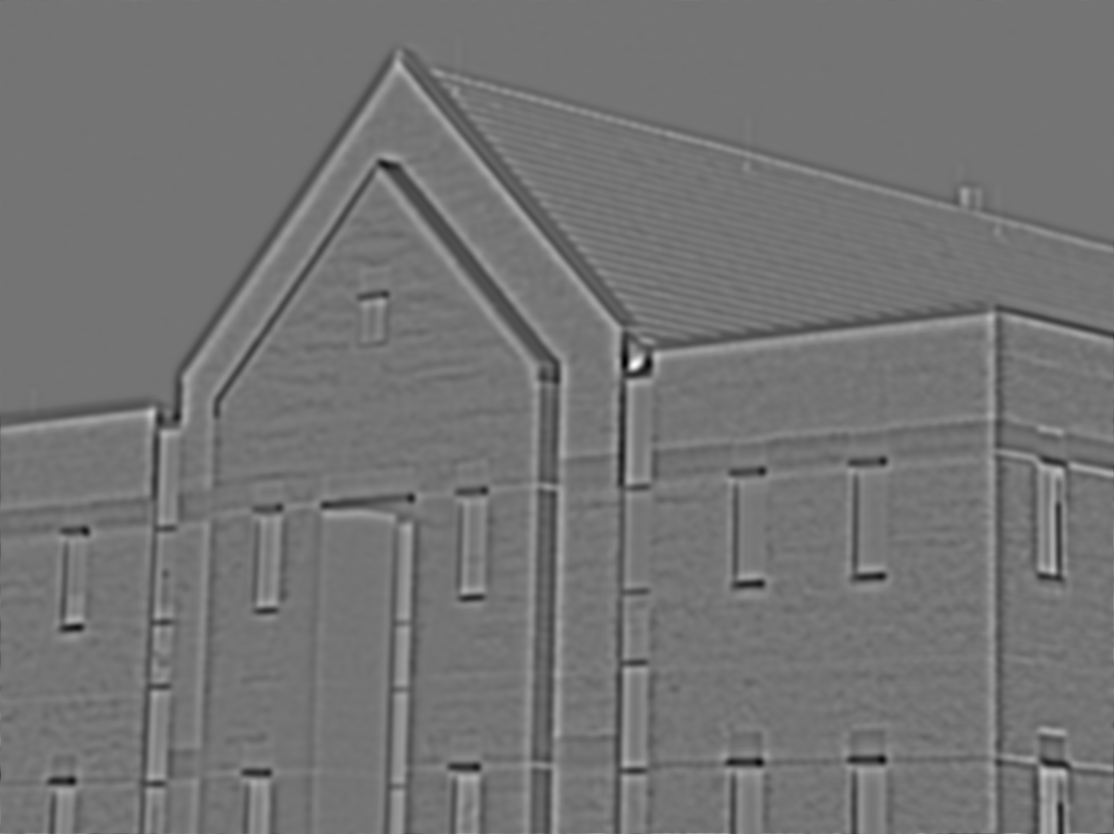
\includegraphics[width=\linewidth]{myfigure/p9/9_marrhildreth.png}
    	\caption{}
    	\label{fig:marrhildreth}
  	\end{subfigure}
  	\begin{subfigure}[b]{0.45\linewidth}
		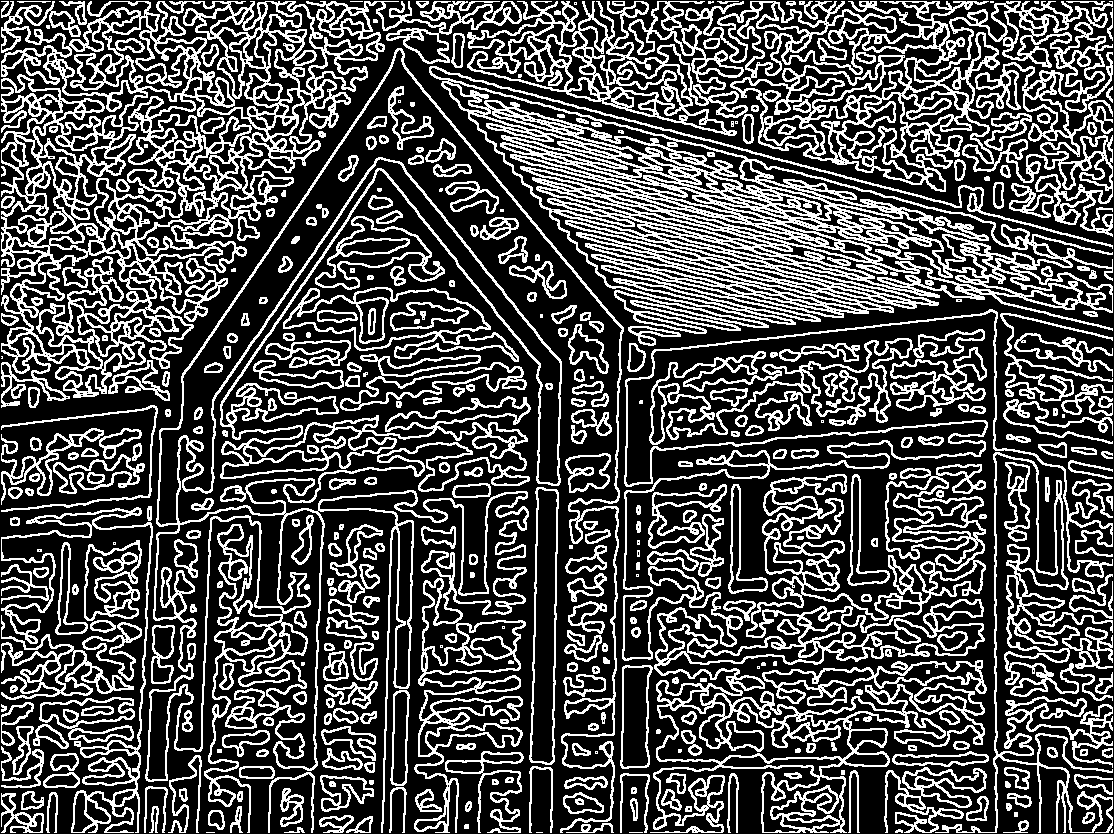
\includegraphics[width=\linewidth]{myfigure/p9/9_zerocross_0.png}
		\caption{}
		\label{fig:zerocross_0}
	\end{subfigure}
	\begin{subfigure}[b]{0.45\linewidth}
		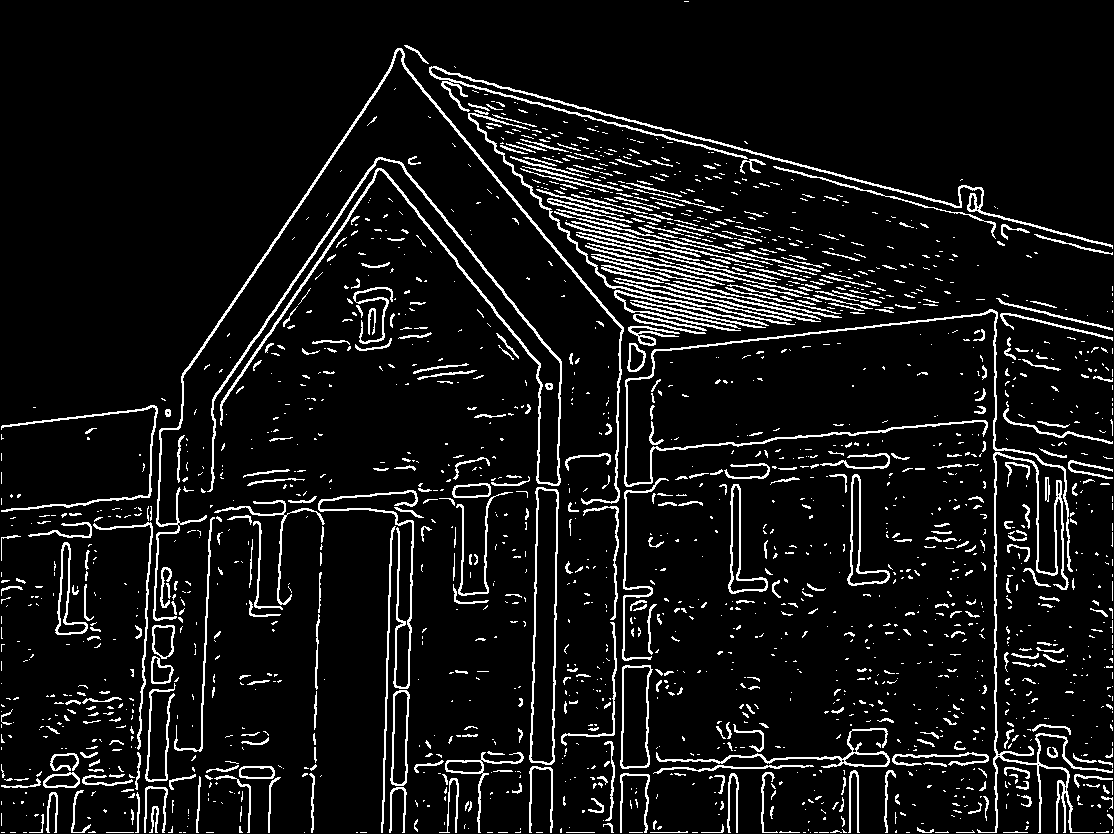
\includegraphics[width=\linewidth]{myfigure/p9/9_zerocross_4.png}
		\caption{}
		\label{fig:zerocross_4}
	\end{subfigure}
	\begin{subfigure}[b]{0.45\linewidth}
		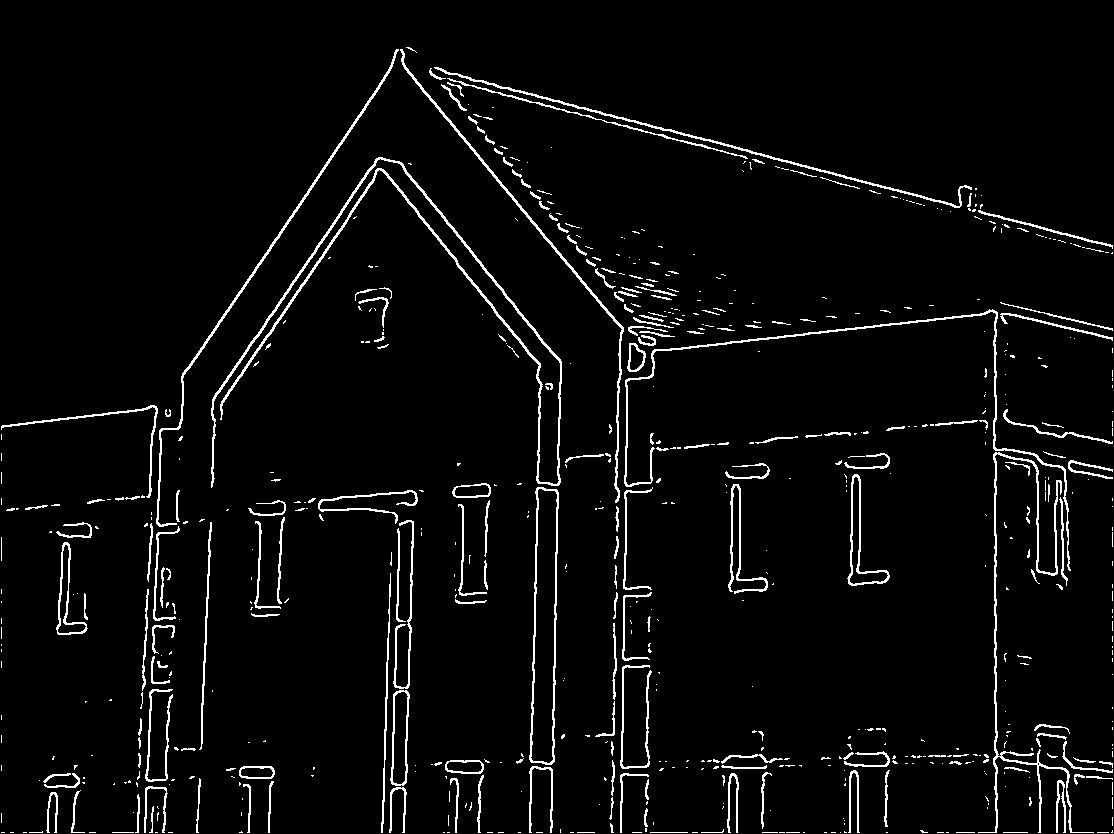
\includegraphics[width=\linewidth]{myfigure/p9/9_zerocross_8.png}
		\caption{}
		\label{fig:zerocross_8}
	\end{subfigure}
	\begin{subfigure}[b]{0.45\linewidth}
		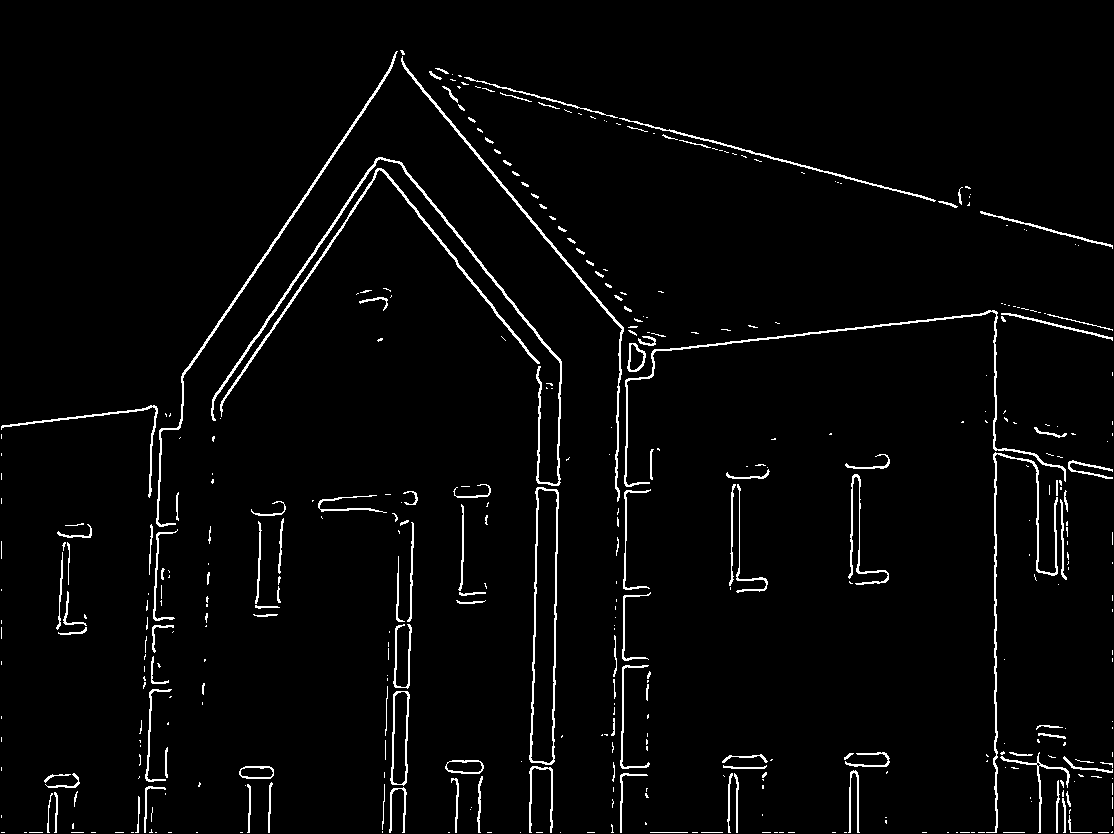
\includegraphics[width=\linewidth]{myfigure/p9/9_zerocross_12.png}
		\caption{}
		\label{fig:zerocross_12}
	\end{subfigure}
	
	\caption{Marr-Hildreth edge detection. \\(a)Original test image of size $834 \times 1115$.\\ (b)Results of Marr-Hildreth(before zero-cross). The gaussian lowpass filter($25\times 25$) used here is with $\sigma=4$.\\  (c)The result of zero cross $threshold=0$.\\ (d)The result of zero cross $threshold=0.04$.\\ (e)The result of zero cross $threshold=0.08$.\\ (f)The result of zero cross $threshold=0.12$.}
  	\label{fig:marr_hildreth}
\end{figure}

Third, I show the process of applying Canny's algorithm in Fig.\ref{fig:eval_canny}. For comparison, Gaussian lowpass filter used here is the same as the one in Marr-Hildreth. The double threshold is $T_H=0.2, T_L=0.1$. We can simply find the Canny's algorithm works better than Marr-Hildreth here. The image in Fig.\ref{fig:thresholdonly} is obtained by use $T_L$, and the result is coarse because of Gaussian smoothing.\\
\begin{figure}[h!]
	\centering
	\begin{subfigure}[b]{0.45\linewidth}
		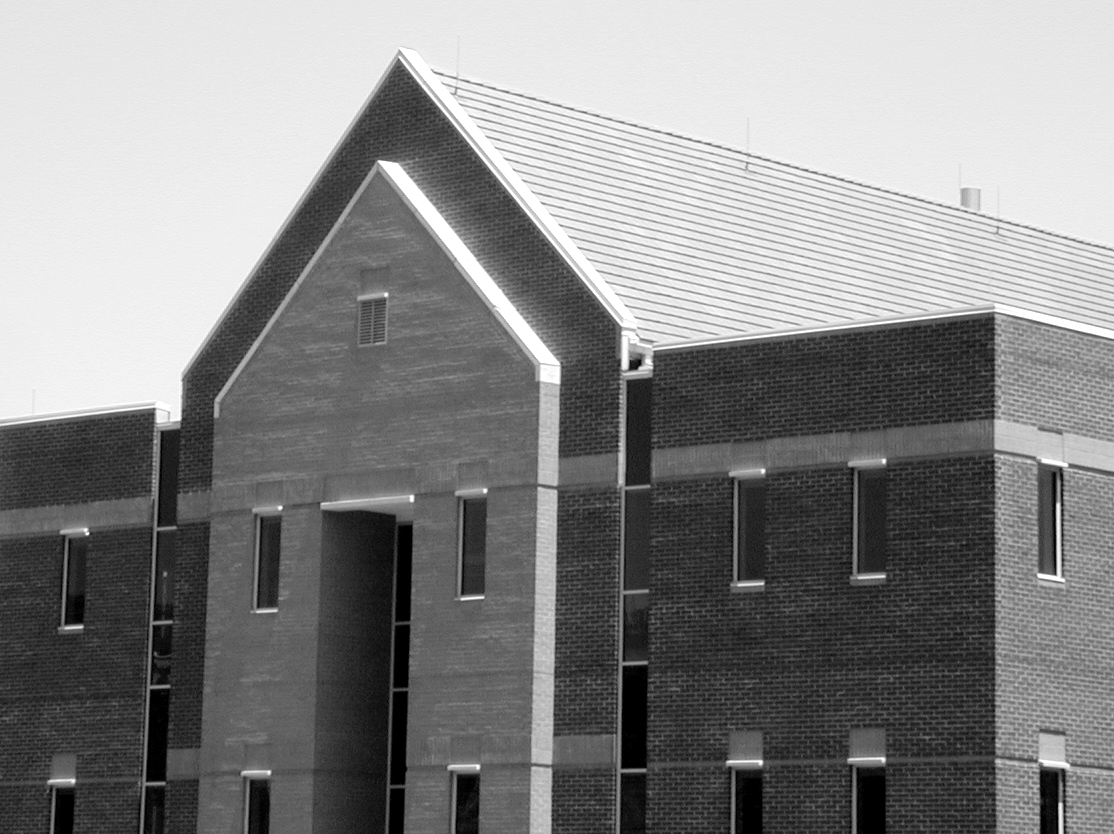
\includegraphics[width=\linewidth]{myfigure/p9/building.png}
		\caption{}
		\label{fig:canny_building}
	\end{subfigure}
	\begin{subfigure}[b]{0.45\linewidth}
    	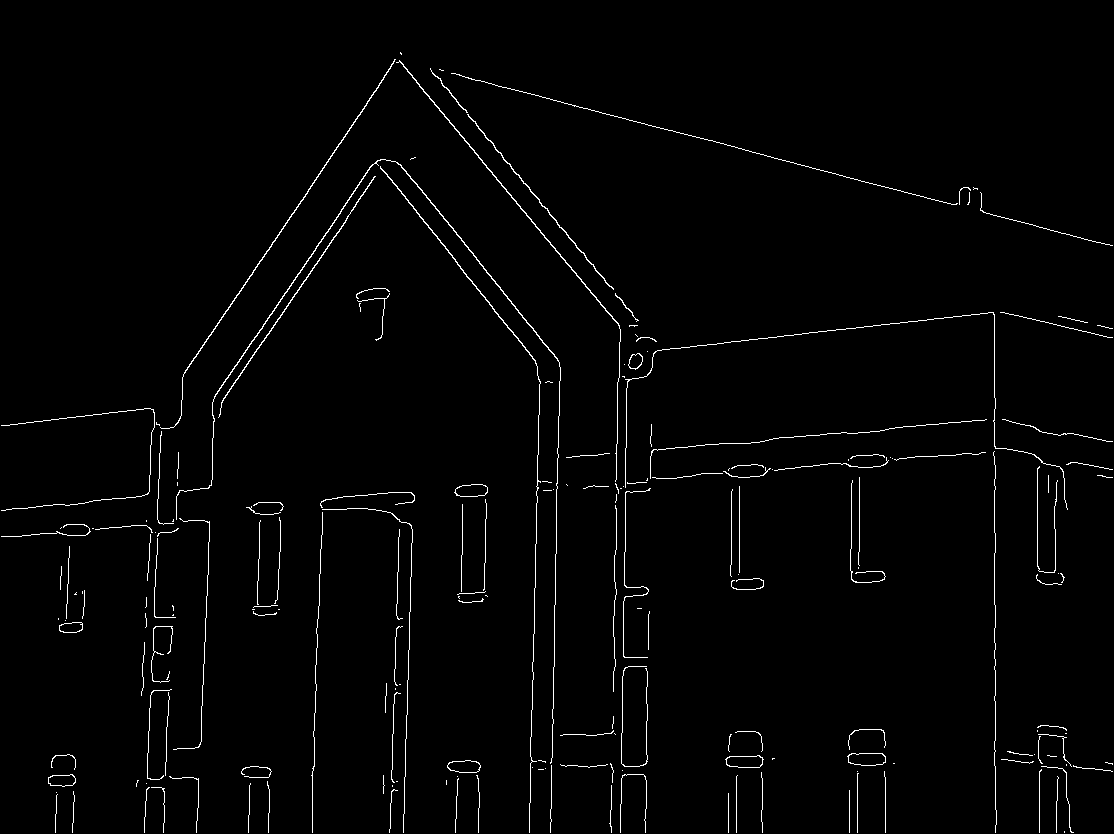
\includegraphics[width=\linewidth]{myfigure/p9/9_threshold_only.png}
    	\caption{}
    	\label{fig:thresholdonly}
  	\end{subfigure}
  	\begin{subfigure}[b]{0.45\linewidth}
		\includegraphics[width=\linewidth]{myfigure/p9/9_zerocross_12.png}
		\caption{}
		\label{fig:zerocross_12_}
	\end{subfigure}
	\begin{subfigure}[b]{0.45\linewidth}
		\includegraphics[width=\linewidth]{myfigure/p9/9_canny.png}
		\caption{}
		\label{fig:canny}
	\end{subfigure}
	
	\caption{Canny edge detection. \\(a)Original test image of size $834 \times 1115$.\\ (b)Use single threshold $T_L$ after Gaussian smoothing. \\(c)Result of Marr-Hildreth(before zero-cross). The Gaussian lowpass filter($25\times 25$) used here is with $\sigma=4$.\\ (d)The result of zero cross $threshold=0.04$.}
  	\label{fig:eval_canny}
\end{figure}

\subsubsection{Global thresholding}
Practice on global thresholding is shown in Fig.\ref{fig:globalthresholding}. The original image is an optical microscope image of polymersome cells. From its histogram, we can see the contrast ratio between foreground and background is low. Hence, it's not surprising the basic global thresholding failed. Using Otsu's method here, we obtain good result. In basic thresholding, I set the $\Delta=1.0$, and obtain $T=169.394997$. In Otse's method, the result is $T=181.000000$ and $Seperability=0.465212$. 
\begin{figure}[h!]
	\centering
	\begin{subfigure}[b]{0.45\linewidth}
		\includegraphics[width=\linewidth]{myfigure/p9/polymersomes.png}
		\caption{}
		\label{fig:polymersomes}
	\end{subfigure}
	\begin{subfigure}[b]{0.45\linewidth}
    	\includegraphics[width=\linewidth]{myfigure/p9/9_polymersomes_hist.png}
    	\caption{}
    	\label{fig:polymersomes_hist}
  	\end{subfigure}
  	\begin{subfigure}[b]{0.45\linewidth}
		\includegraphics[width=\linewidth]{myfigure/p9/9_threshold_basic.png}
		\caption{}
		\label{fig:threshold_basic}
	\end{subfigure}
	\begin{subfigure}[b]{0.45\linewidth}
		\includegraphics[width=\linewidth]{myfigure/p9/9_threshold_otsu.png}
		\caption{}
		\label{fig:threshold_otsu}
	\end{subfigure}
	
	\caption{Global thresholding. \\(a)Original test image (b)Histogram of the test image. \\(c)Basic thresholding end with $T=169.394997$\\ (d)Otsu's method end with $T=181.000000, sepearablity=0.465212$.}
  	\label{fig:globalthresholding}
\end{figure}

\clearpage
\subsection{Implementation}
Here list the function implemented in this project. They are \emph{roberts, prewitt, sobel, marr\_hildreth, canny, basic\_global\_thresholding, otsu\_thresholding}.

\lstset{language=Matlab}
\begin{lstlisting}
function [ imgg ] = roberts( imgf )
%ROBERTS 
%   robert filter, two with 3x3 masks on axis-x and axis-y

[M, N] = size(imgf);

f = replicate_padding(imgf, 2);
f = double(f); % double f

% Roberts
maskx = [0 0 0 ; 0 -1 0; 0 0 1];
masky = [0 0 0; 0 0 -1; 0 1 0];

gx = zeros(M+4, N+4);
gy = zeros(M+4, N+4);

for x = (2 : M+3)
    for y = (2 : N+3)
        gx(x, y) = sum(sum(f(x-1:x+1, y-1:y+1) .* maskx));
        gy(x, y) = sum(sum(f(x-1:x+1, y-1:y+1) .* masky));
    end
end

% new image: using abs ,some negative
gx = abs(gx(3:M+2, 3:N+2));
gy = abs(gy(3:M+2, 3:N+2));
imgg = scale255(gx+gy);

end
\end{lstlisting}

\lstset{language=Matlab}
\begin{lstlisting}
function [ imgg ] = prewitt( imgf )
%PREWITT prewitt filter
%   two 3x3 masks

[M, N] = size(imgf);

f = replicate_padding(imgf, 2);
f = double(f); % double f

maskx = [-1 -1 -1; 0 0 0; 1 1 1];
masky = [-1 0 1; -1 0 1; -1 0 1];

gx = zeros(M+4, N+4);
gy = zeros(M+4, N+4);

for x = (2 : M+3)
    for y = (2 : N+3)
        gx(x, y) = sum(sum(f(x-1:x+1, y-1:y+1) .* maskx));
        gy(x, y) = sum(sum(f(x-1:x+1, y-1:y+1) .* masky));
    end
end

% new image: using abs ,some negative
gx = abs(gx(3:M+2, 3:N+2));
gy = abs(gy(3:M+2, 3:N+2));
imgg = scale255(gx+gy);

end
\end{lstlisting}
 
 \lstset{language=Matlab}
\begin{lstlisting}
function [ imgg ] = sobel( imgf )
%SOBEL 

[M, N] = size(imgf);

f = replicate_padding(imgf, 2);
f = double(f); % double f

% Sobel
maskx = [-1 -2 -1; 0 0 0; 1 2 1];
masky = [-1 0 1; -2 0 2; -1 0 1];
gx = zeros(M+4, N+4);
gy = zeros(M+4, N+4);
for x = (2 : M+3)
    for y = (2 : N+3)
        gx(x, y) = sum(sum(f(x-1:x+1, y-1:y+1) .* maskx));
        gy(x, y) = sum(sum(f(x-1:x+1, y-1:y+1) .* masky));
    end
end

% new image: using abs
gx = abs(gx(3:M+2, 3:N+2));
gy = abs(gy(3:M+2, 3:N+2));
imgg = scale255(gx+gy);

end
\end{lstlisting}

\lstset{language=Matlab}
\begin{lstlisting}
function [ imgg, imgcross ] = marr_hildreth( imgf, sigma, n, threshold )
%MARR_HILDRETH 
%   sigma - variance of Gaussian, n - size of gaussiain lowpass filter

% generate gaussian filter
x = (1:n) - (n+1)/2;
y = x';
x = repmat(x, n, 1);
y = repmat(y, 1, n);
D2 = x.^2 + y.^2;
gau_filter = exp(-D2 / (2*sigma*sigma));

% preprocess
[M, N] = size(imgf);
imgf = double(imgf) ./ 255;
f = replicate_padding(imgf, n-1);
f = double(f); % double f

% convolution
g = zeros(M+2*n, N+2*n);
for x = (n : M+n-1)
    for y = (n : N+n-1)
        xlow = fix(x - fix((n-1)/2));
        xhigh = fix(x + fix((n-1)/2));
        ylow = fix(y - fix((n-1)/2));
        yhigh = fix(y + fix((n-1)/2));
        g(x,y) = sum(sum(f(xlow:xhigh,ylow:yhigh) .* gau_filter));
    end
end

f = g(n:M+n-1, n:N+n-1) * 255;
% laplacian
f = replicate_padding(f, 2);
mask = [1 1 1; 1 -8 1; 1 1 1];
g = zeros(M+4, N+4);
for x = (2 : M+3)
    for y = (2 : N+3)
        g(x, y) = sum(sum(f(x-1:x+1, y-1:y+1) .* mask));
    end
end

% do zero cross
g = g(3:M+2, 3:N+2);
imgcross = zero_cross(g, threshold*max(max(g)));

imgg = g; % laplacian result without scale
imgg = scale255(imgg); % this is the image to show
imgcross = scale255(imgcross);

end
\end{lstlisting}

\lstset{language=Matlab}
\begin{lstlisting}
function [ imgg, imgt ] = canny( imgf, sigma, n, TL, TH )
%CANNY canny's algorithm
%   sigma - gaussian variance, n - size of filter, TH TL - thresholds

% generate gaussian filter
x = (1:n) - (n+1)/2;
y = x';
x = repmat(x, n, 1);
y = repmat(y, 1, n);
D2 = x.^2 + y.^2;
gau_filter = exp(-D2 / (2*sigma*sigma));

% preprocess
[M, N] = size(imgf);
imgf = double(imgf) ./ 255;
f = replicate_padding(imgf, n-1);
f = double(f); % double f

% gaussian smoothing
g = zeros(M+2*n, N+2*n);
for x = (n : M+n-1)
    for y = (n : N+n-1)
        xlow = fix(x - fix((n-1)/2));
        xhigh = fix(x + fix((n-1)/2));
        ylow = fix(y - fix((n-1)/2));
        yhigh = fix(y + fix((n-1)/2));
        g(x,y) = sum(sum(f(xlow:xhigh,ylow:yhigh) .* gau_filter));
    end
end

% restore to original size
f = g(n:M+n-1, n:N+n-1);
minf = min(min(f));
maxf = max(max(f));
f = (f - minf)./(maxf-minf); % normalization to (0,1)

% calculate magnitude and angle image
magnitude = zeros(M, N);
angle = zeros(M, N);
for x = (1:M-1)
    for y = (1:N-1)
        py = f(x,y) - f(x,y+1) + f(x+1,y) - f(x+1,y+1);
        px = f(x,y) - f(x+1,y) + f(x,y+1) - f(x+1,y+1);
        magnitude(x, y) = sqrt(px*px + py*py);
        angle(x, y) = atand(py/px);
    end
end

% obtain thresholding-only image
imgt = zeros(M, N);
for x = (1:M)
    for y = (1:N)
        if magnitude(x,y)>=TL 
            imgt(x,y) = magnitude(x,y);
        end
    end
end
imgt = uint8(scale255(imgt));

% nonmaximum suppression
suppres = zeros(M, N);

for x = (2:M-1)
    for y = (2:N-1)
        if angle(x,y)>=-22.5 && angle(x,y)<22.5 % horizontal
            if magnitude(x,y)>magnitude(x-1,y) && magnitude(x,y)>magnitude(x+1,y)
                suppres(x, y) = magnitude(x,y);
            end
        elseif angle(x,y)>=22.5 && angle(x,y)<67.5 % leftbottom-righttop
            if magnitude(x,y)>magnitude(x-1,y-1) && magnitude(x,y)>magnitude(x+1,y+1)
                suppres(x, y) = magnitude(x,y);
            end
        elseif angle(x,y)>=-67.5 && angle(x,y)<-22.5 % lefttop-rightbottom
            if magnitude(x,y)>magnitude(x-1,y+1) && magnitude(x,y)>magnitude(x+1,y-1)
                suppres(x, y) = magnitude(x,y);
            end
        else % vertical
            if magnitude(x,y)>magnitude(x,y+1) && magnitude(x,y)>magnitude(x,y-1)
                suppres(x, y) = magnitude(x,y);
            end
        end
    end
end

% double thresholding
imgg = zeros(M, N);

for x = (1:M)
    for y = (1:N)
        if suppres(x,y)>TH % strong edge pixel
            imgg(x,y) = 1;
        elseif suppres(x,y)>TL 
            if max(max(suppres(x-1:x+1,y-1:y+1)))>TH % 8-connectivity
                imgg(x,y) = 1;
            end
        end            
    end
end

end
\end{lstlisting}

\lstset{language=Matlab}
\begin{lstlisting}
function [ imgg, T ] = basic_global_thresholding( imgf, T0, deltaT )
%BASIC_GLOBAL_THRESHOLDING 
%   T0: init esitimatation threshold, deltaT: the stopping difference

while 1
    [~, mean_0, mean_1] = thresholding(imgf, T0);
    T1 = (mean_0+mean_1)/2;
    if abs(T1-T0) <= deltaT
        T = T1;
        break
    end
    T0 = T1;
end
[imgg, ~, ~] = thresholding(imgf, T);

end

function [ imgg, mean_0, mean_1 ] = thresholding( imgf, T )    
[M, N] = size(imgf);
imgg = zeros(M, N);
mean_0 = double(0);
mean_1 = double(0);
cnt_0 = 0;
cnt_1 = 0;
for x = (1:M)
    for y = (1:N)
        if imgf(x,y)>T
            imgg(x,y)=250;
            mean_1 = mean_1+double(imgf(x,y));
            cnt_1 = cnt_1+1;
        else
            imgg(x,y)=5;
            mean_0 = mean_0+double(imgf(x,y));
            cnt_0 = cnt_0+1;
        end
    end
end

imgg = uint8(imgg);
if mean_0 == 0
    cnt_0 = 1;
end
if mean_1 == 0
    cnt_1 = 1;
end

mean_0 = mean_0 / cnt_0;
mean_1 = mean_1 / cnt_1;

end
\end{lstlisting}

\lstset{language=Matlab}
\begin{lstlisting}
function [ imgg, kstar, eta ] = otsu_thresholding( imgf )
%OTSU_THRESHOLDING 
%   kstar: threshold, eta: separability

[M, N] = size(imgf);
histf = zeros(1, uint32(256)); % (0:255)
for x=(1:M)
    for y=(1:N)
        histf(fix(imgf(x,y)+1)) = histf(fix(imgf(x,y)+1)) + 1;
    end
end
histf = double(histf)/double(M*N);

P = zeros(1, uint32(256));
P(1) = histf(1);
for i = (2:256)
    P(i) = P(i-1) + histf(i);
end

m = double(zeros(1, uint32(256)));
m(1) = 0*double(histf(1));
for i = (2:256)
    m(i) = m(i-1) + double(i-1)*histf(i);
end
mG = m(256);

size(P)
size(m)
size(mG)
size(1-P)

sigmaB2 = (mG .* P - m) .^2 ./(P .* (1-P));
size(sigmaB2)
kall = find(sigmaB2==max(sigmaB2));
kstar = mean(kall) - 1;
sigmaG = sum(((0:255)-mG).^2 .* histf);

eta = sigmaB2(int32(kstar)) / sigmaG;
imgg = thresholding(imgf, kstar);

end

function [ imgg ] = thresholding( imgf, T )    
[M, N] = size(imgf);
imgg = zeros(M, N);
for x = (1:M)
    for y = (1:N)
        if imgf(x,y)>T
            imgg(x,y)=250;
        else
            imgg(x,y)=5;
        end
    end
end

imgg = uint8(imgg);
end
\end{lstlisting}



\end{document}